\documentclass[../document.tex]{subfiles}
\begin{document}
\chapter{Results}
\label{chap: results}
In the section we show and evaluate the model's results. We will start by presenting to the reader the networks score on each metric, then we will use the best model to predict the traversability in real world terrains. 
\section{Experiment setup}
% \subsection{Hardware}
We run all the experiment on a Ubuntu 18.10  work station equipped with a Ryzen 2700x, a powerful CPU with 8 cores and 16 threads, and a NVIDIA 1080 GPU with 8GB of dedicated RAM.
\section{Dataset}
To perform classification, we select a threshold of $0.2$m on a time window, $\Delta t$, of two seconds to label the patches, meaning that a patch with an advancement less than $20$ centimeters is labeled as \emph{no traversable} and viceversa. This processed is explained in detail in the previous chapter. While for the regression, we did not label the patch and directly regress on the advancement.

Initially, to train the models we first use Standard Gradient Descent with momentum set to $0.95$, weight decay to $1e-4$ and an initial learning rate of $1e-3$ as was originally proposed in He et al. \cite{he2015deep}. However, we later utilize Leslie Smith's 1cycle policy \cite{1cycle} that allows us to trian the network faster and with an higher accuracy. We minimise the binary Cross Entropy for the classifier and the  Mean Square Error (MSE) for the regressor.
\subsection{Experimental validation}
We select as \emph{validation} set ten percent of the training data. Since we store each run of Krock as a \emph{.csv} file, validation and train set do not overlap. 
The test set is composed entirely by the Quarry map, a real world scenario. Table \ref{table: maps} tells in detail the configuration used in each map of all sets.

We also evaluate the model on the following additonal maps
\todo[inline]{ add arck rocks}
\subsection{Metrics}

\paragraph{Classification:} To evaluate the model's classification performance we used two metrics: \emph{accuracy} and \emph{AUC-ROC Curve}. Accuracy scores the number of correct predictions made by the network while AUC-ROC Curve represents degree or measure of separability, informally it tells how much model is capable of distinguishing between classes. For each experiment, we select the model with the higher AUC-ROC Curve during training to be evaluated on the test set.



\paragraph{Regression:} We used the Mean Square Error to evaluate the model's performance.
\section{Quantitative results}
\subsection{Model selection}
We compared two different \emph{micro-resnet} and the \emph{vanilla} cnn from the previous Chapter. We evaluate those models using a time window of two second, a threshold of $20$cm and the data augmentation techniques described before. We run five experiments per architecture and we select the best performing network, the results are showed in the following table. 

\begin{table*}[ht]
  \centering
  \ra{1.2}
  \begin{tabular}{@{}lcccc@{}}
  \toprule
   && Vanilla & \multicolumn{2}{c}{MicroResnetSE} \\
  \cline{3-5}
  && & $3\times 3$ stride $1$ & $7\times7$ stride $2$\\ 
  \cline{3-5}
  \multirow{2}{*}{AUC} & Top & 0.892 & 0.888 & \textbf{0.896}\\
   & Mean & \textbf{0.890} & 0.883 & 0.888\\
  \cline{1-5}
  Params & & 974,351 & 313,642 & 314,282  \\
  \bottomrule   
\end{tabular}
\caption{Model comparison on the test set.}
\end{table*}
\todo[inline]{Luca told me is better to split the models like Model1 and Model2 etc}

Based on this data We select \emph{micro-resnet} with squeeze and excitation and a starting convolution's kernel size of $7\times7$ with stride of $2$. This model has one third of the parameter of the origal model proposed by Chavez-Garcia et all \cite{omar2018traversability}. 

As proof of work, we also train the best network architecture, MicroResnetSE with a first convolution's kernel size of $7 \times 7$ and stride$=2$, with and without the Squeeze and Excitation operator.
\begin{table*} [htbp]
  \centering
  \ra{1.2}
  \begin{tabular}{@{}lccc@{}}
  \toprule
  &  MicroResnet$7\times7$ & MicroResnet$7\times7$-SE  & Improvement \\
  \cline{1-4}
   Top & 0.875 & \textbf{0.896} & $+0.021$ \\
   Mean & 0.867 & \textbf{0.888} & $+0.021$ \\
  \bottomrule   
\end{tabular}
\caption{AUC top value and mean value for MicroResnet with a fist convolution of $7\times7$ and stride $=2$ with and without the SE module. The improvement is the same.}
\end{table*}

\section{Final results}
\subsubsection{Classification}
Table \ref{tab : classification-results} table shows in deep the score of the best network for each dataset. We obtained $95\%$ accuracy and $0.96$ AUC on the validation set and $88\%$ accuracy and $0.89$ AUC on the test set.
\begin{table*}[htbp]
    \centering
    \ra{1.2}
    \begin{tabular}{@{}llccccc@{}}
    \toprule
    % \multicolumn{8}{c}{Quantitative evaluation in simulation} \\
    \multicolumn{2}{c}{Dataset} && \multicolumn{2}{c}{micro-resnet} & Size & Resolution(cm/px) \\
    \cmidrule{1-2} \cmidrule{4-5}
    Type     &  Name  & Samples & ACC  &  AUC    & & \\
    \toprule
      \multirow{3}{*}{Synthetic}  & Training   & 429312 & - & - & & 2\\
      &  Validation   & 44032 &  95.2 \% &  0.961 & & 2 \\
      & Arc Rocks & 37273 &  85.5 \% &  0.888 & & 2 \\
      \cmidrule{2-7}
    \multirow{3}{*}{\makecell[l]{Real\\evaluation}} & Quarry & 36224 &  88.2 \%&  0.896& & 2\\
    \bottomrule   
\end{tabular}
\caption{Classification results on different datasets.}
\label{tab : classification-results}
\end{table*}
% Moreover, we would like to also show the different steps we made to reach this result. The following table shows the metric's score without any data-augmentation.
% Adding dropout increases the results.
% With dropout plus coarse dropout.
\section{Qualitative results}
We qualitative evaluate the model predictions by plotting the traversability probability on different maps in 3D.  We used a sliding window to extract the patches from the tested maps to collect the model's predictions. Then, we created a texture based on the traversable probability, we have colored it using a colormap and finally applied on the 3D model of each map. We evaluated four rotations, from bottom to top, top to bottom, left to right and right to left since those are the most human understandable. By using those angles, we can optimize the cropping process since there is not need to rotate each patch based on the Krock's head position. Instead, we can just rotate the entire map beforehand. 
\subsection{Quarry}
The first map we evaluate is Quarry, this map is $32\times 32$m long and has a maximum height of $10$m. We can use some of the terrain interesting features, such as are three bis slopes and the rocky ground on top, to evaluate the model. For instance, w expect the trail on the slopes to be traversable at almost any rotation, expecially from left to right and viceversa. While, the top part should be hard to traverse in almost any case. The following figure shows the traversability probability directly on the map. 
\todo[inline]{some where place the colormap bar}
\begin{figure} [htbp]
\centering
\begin{subfigure}[b]{0.45\textwidth}
  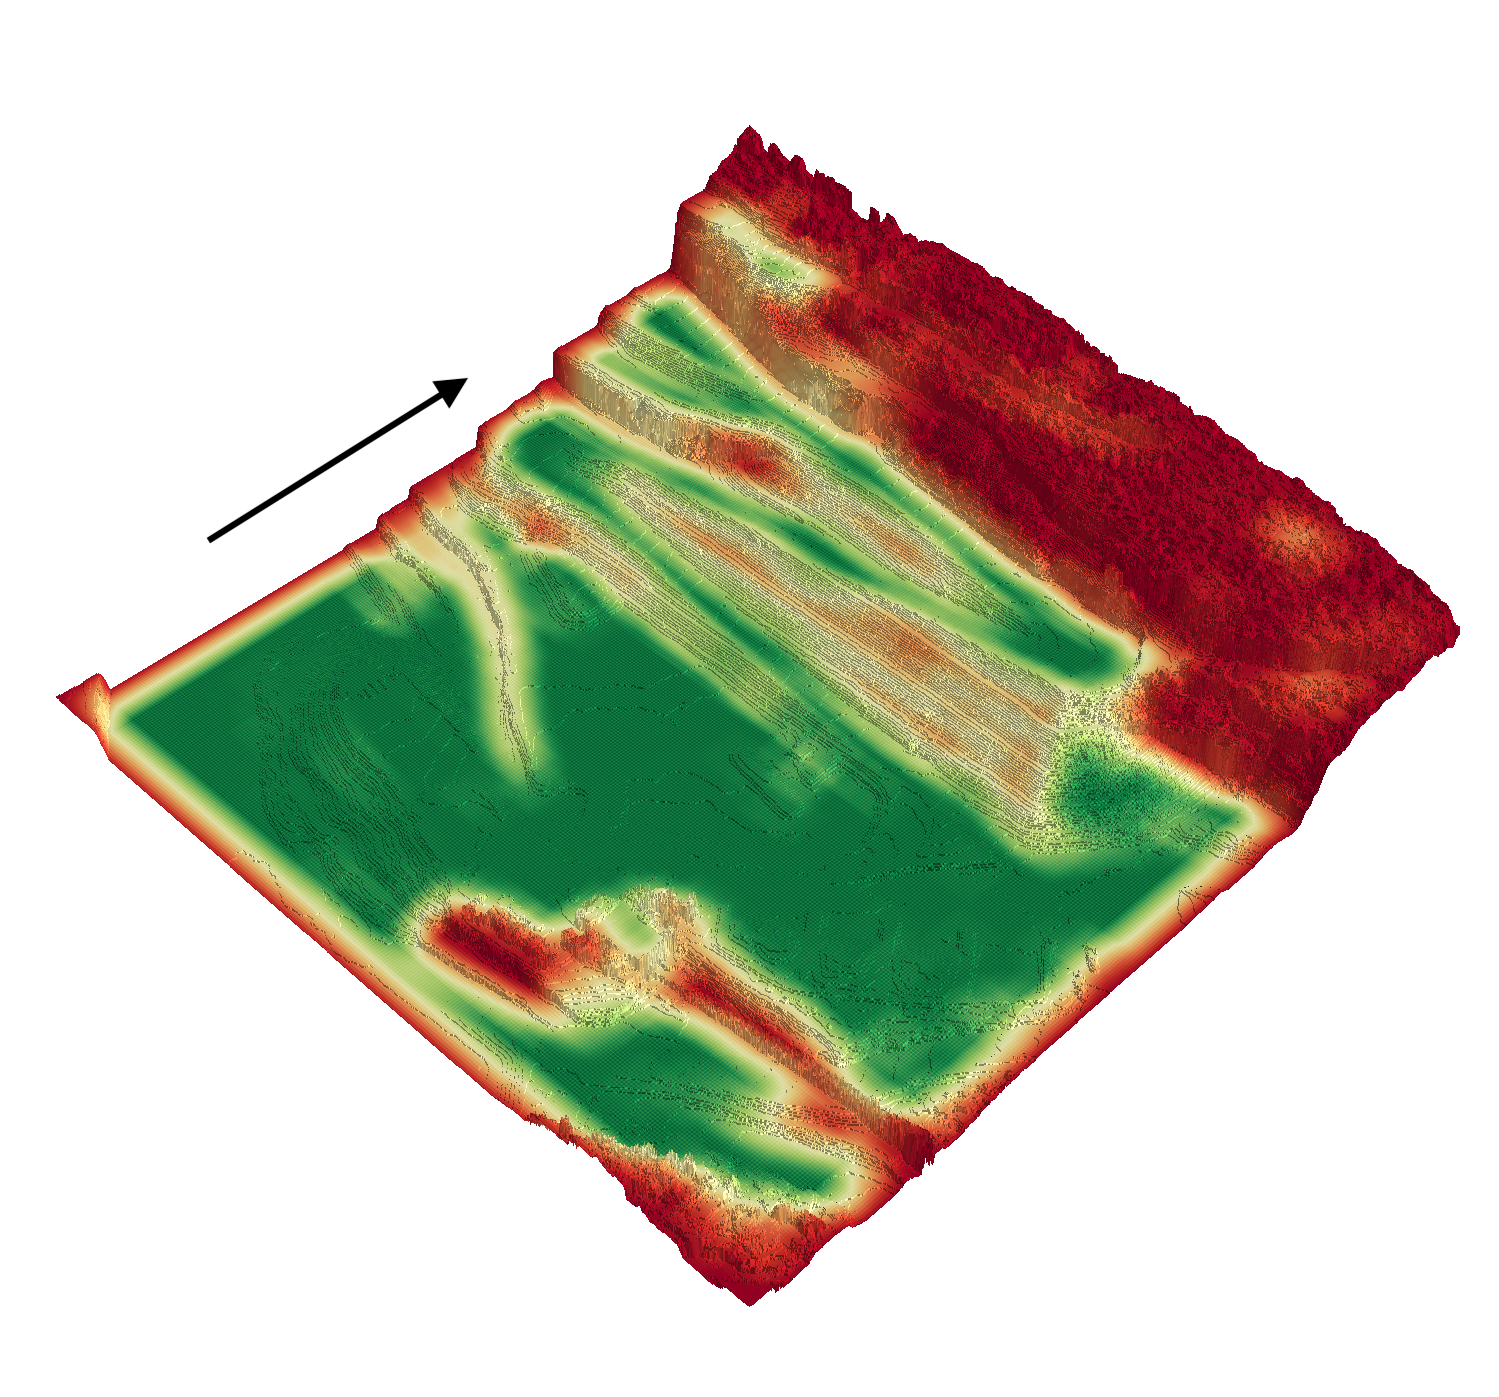
\includegraphics[width=\linewidth]{../img/4/traversability/quarry/-270.png} 
  \subcaption{Robot moving from bottom to top} 
  % \label{fig: quarry-b2t}
\end{subfigure}
\begin{subfigure}[b]{0.45\textwidth}
    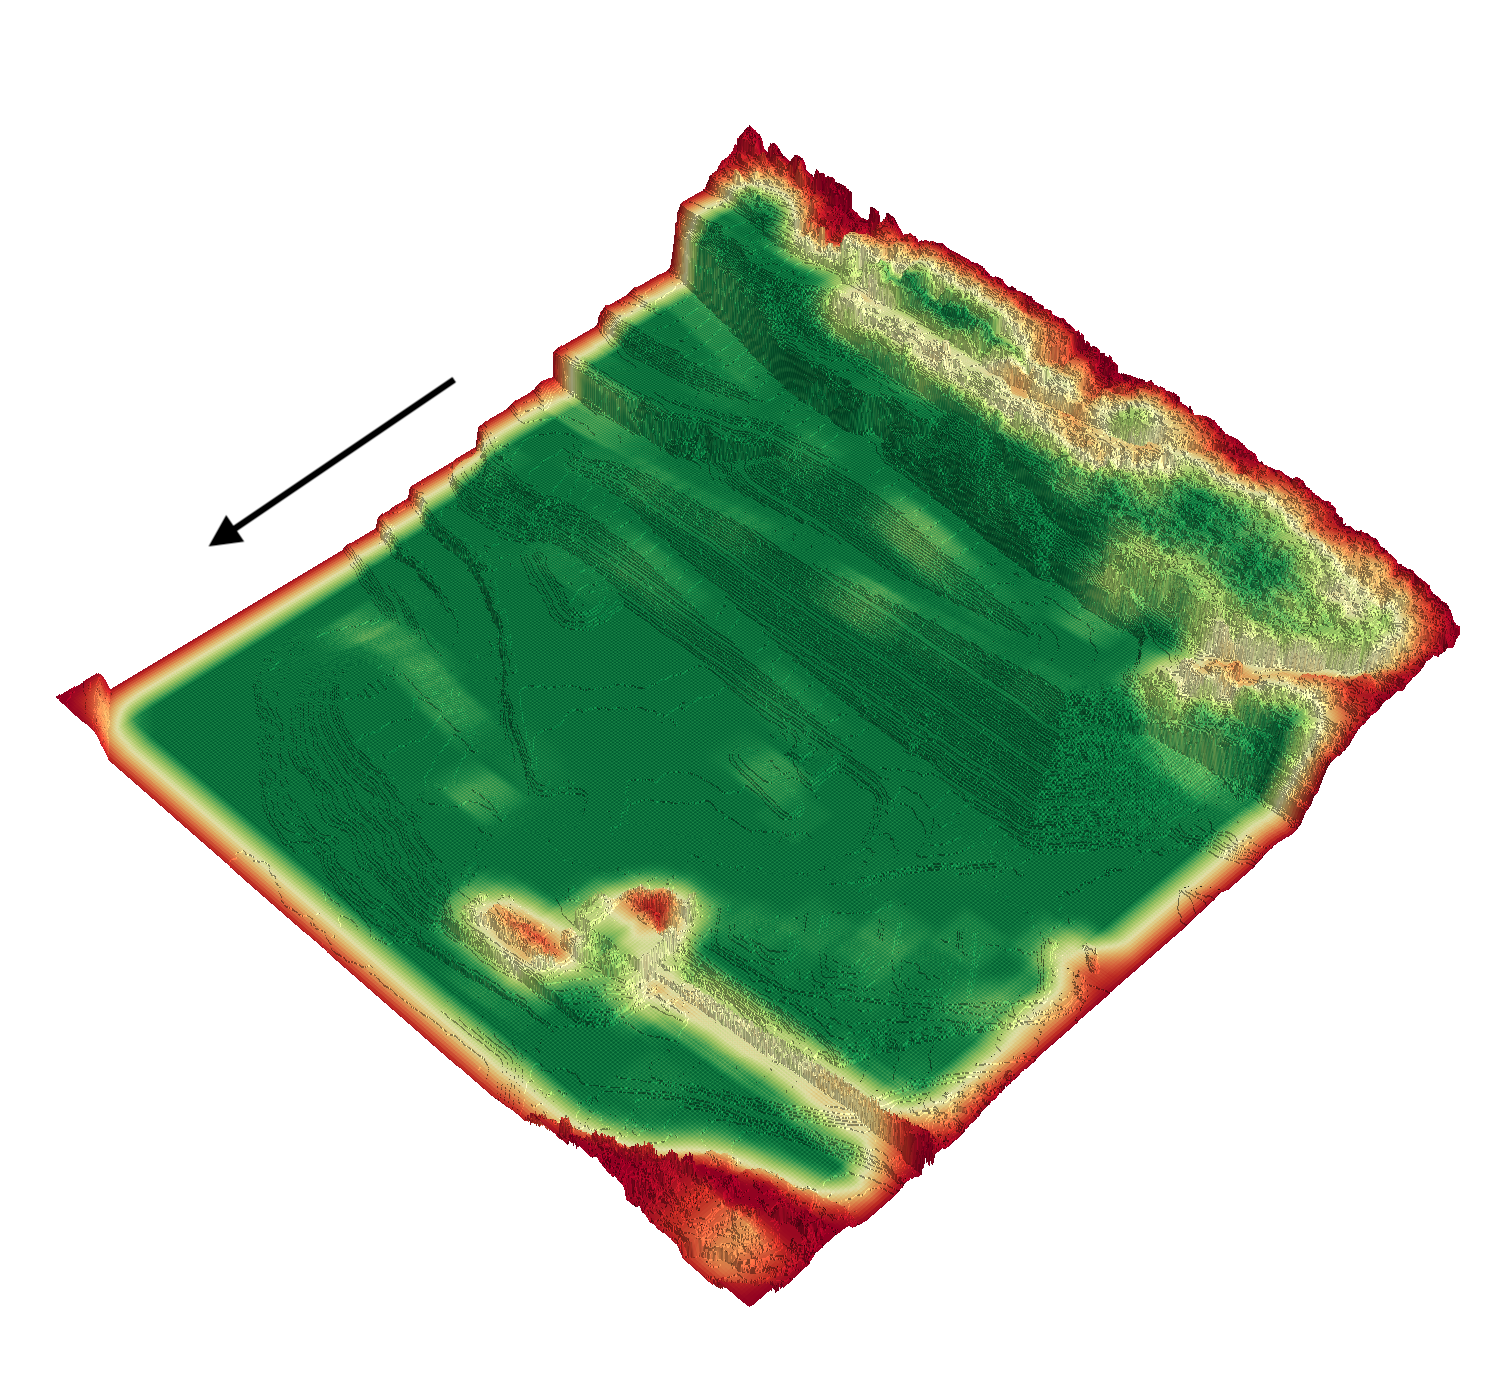
\includegraphics[width=\linewidth]{../img/4/traversability/quarry/-90.png}
    \subcaption{Robot moving from top to bottom} 
    % \label{fig: quarry-t2b}
\end{subfigure}
\begin{subfigure}[b]{0.45\textwidth}
  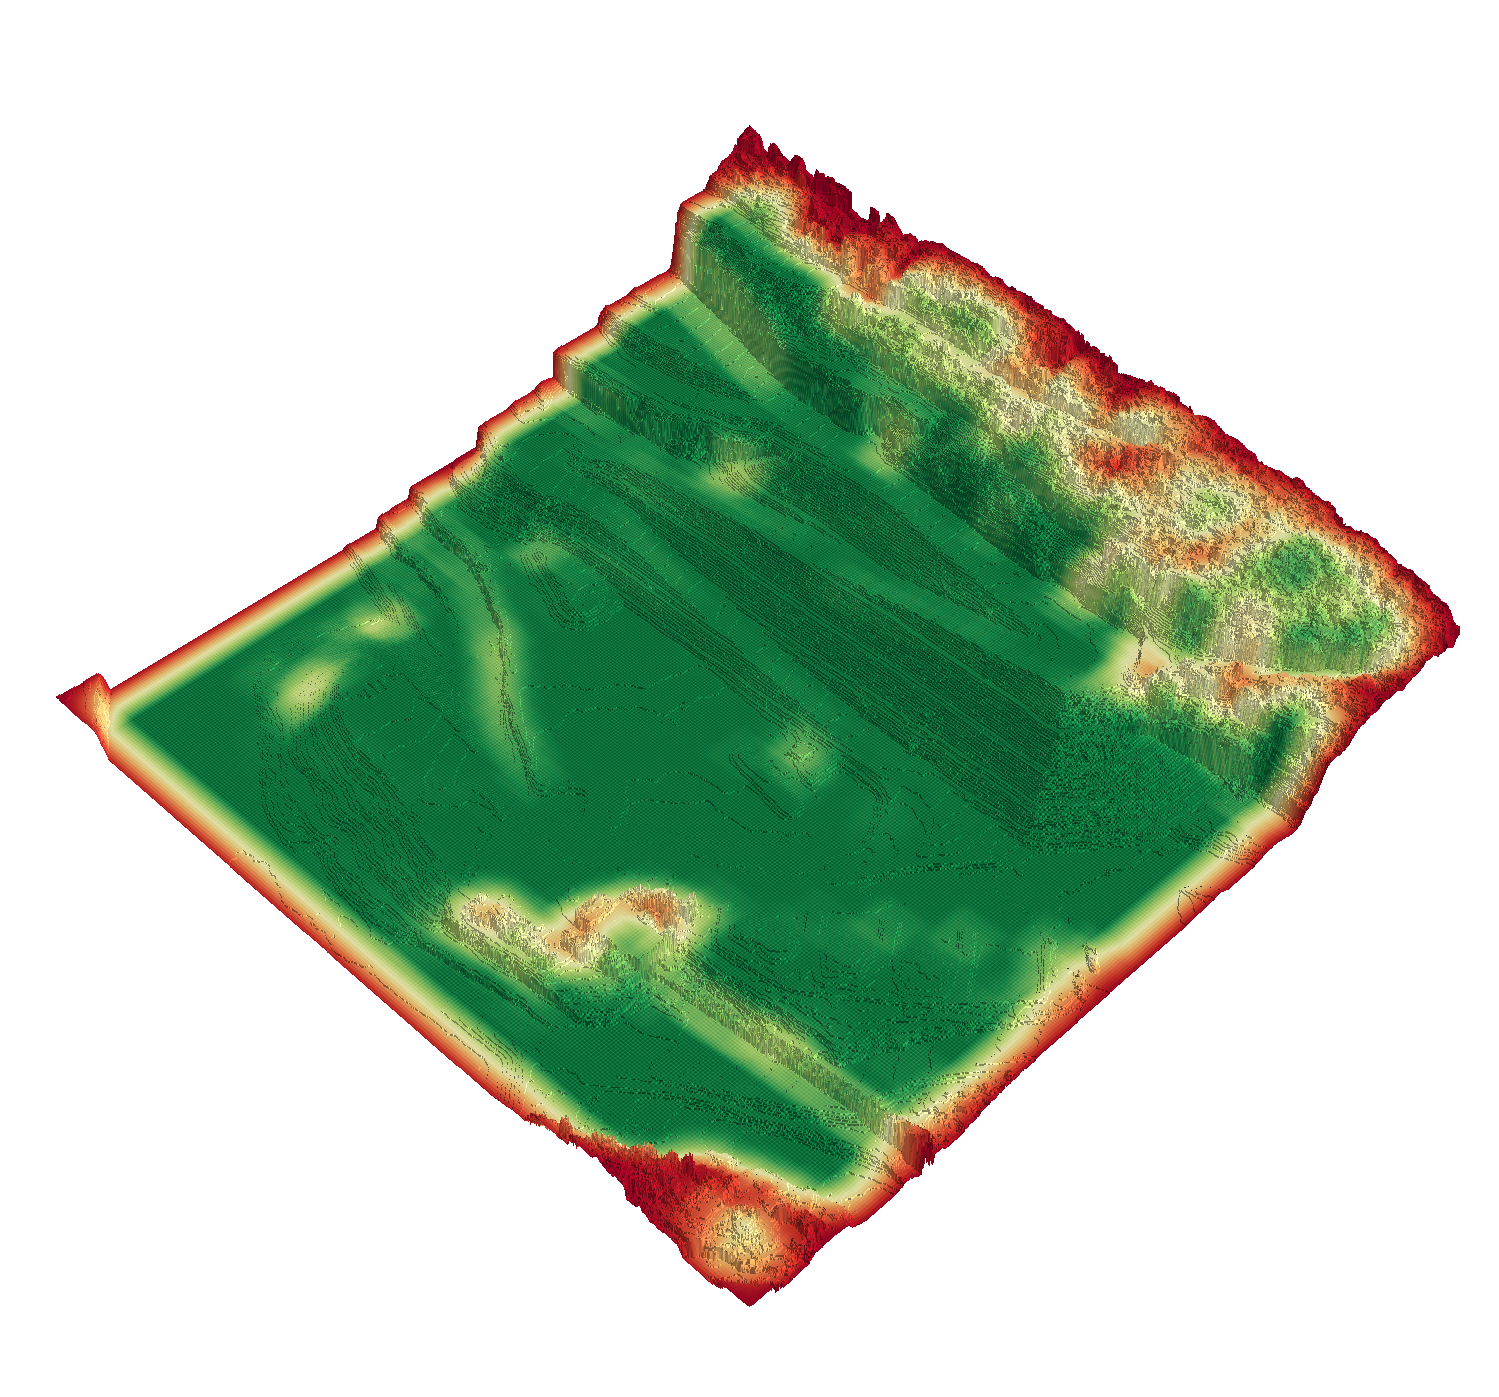
\includegraphics[width=\linewidth]{../img/4/traversability/quarry/-0.png}
  \subcaption{Robot moving from left to right}   
  % \label{fig: quarry-l2r}
\end{subfigure}
\begin{subfigure}[b]{0.45\textwidth}
    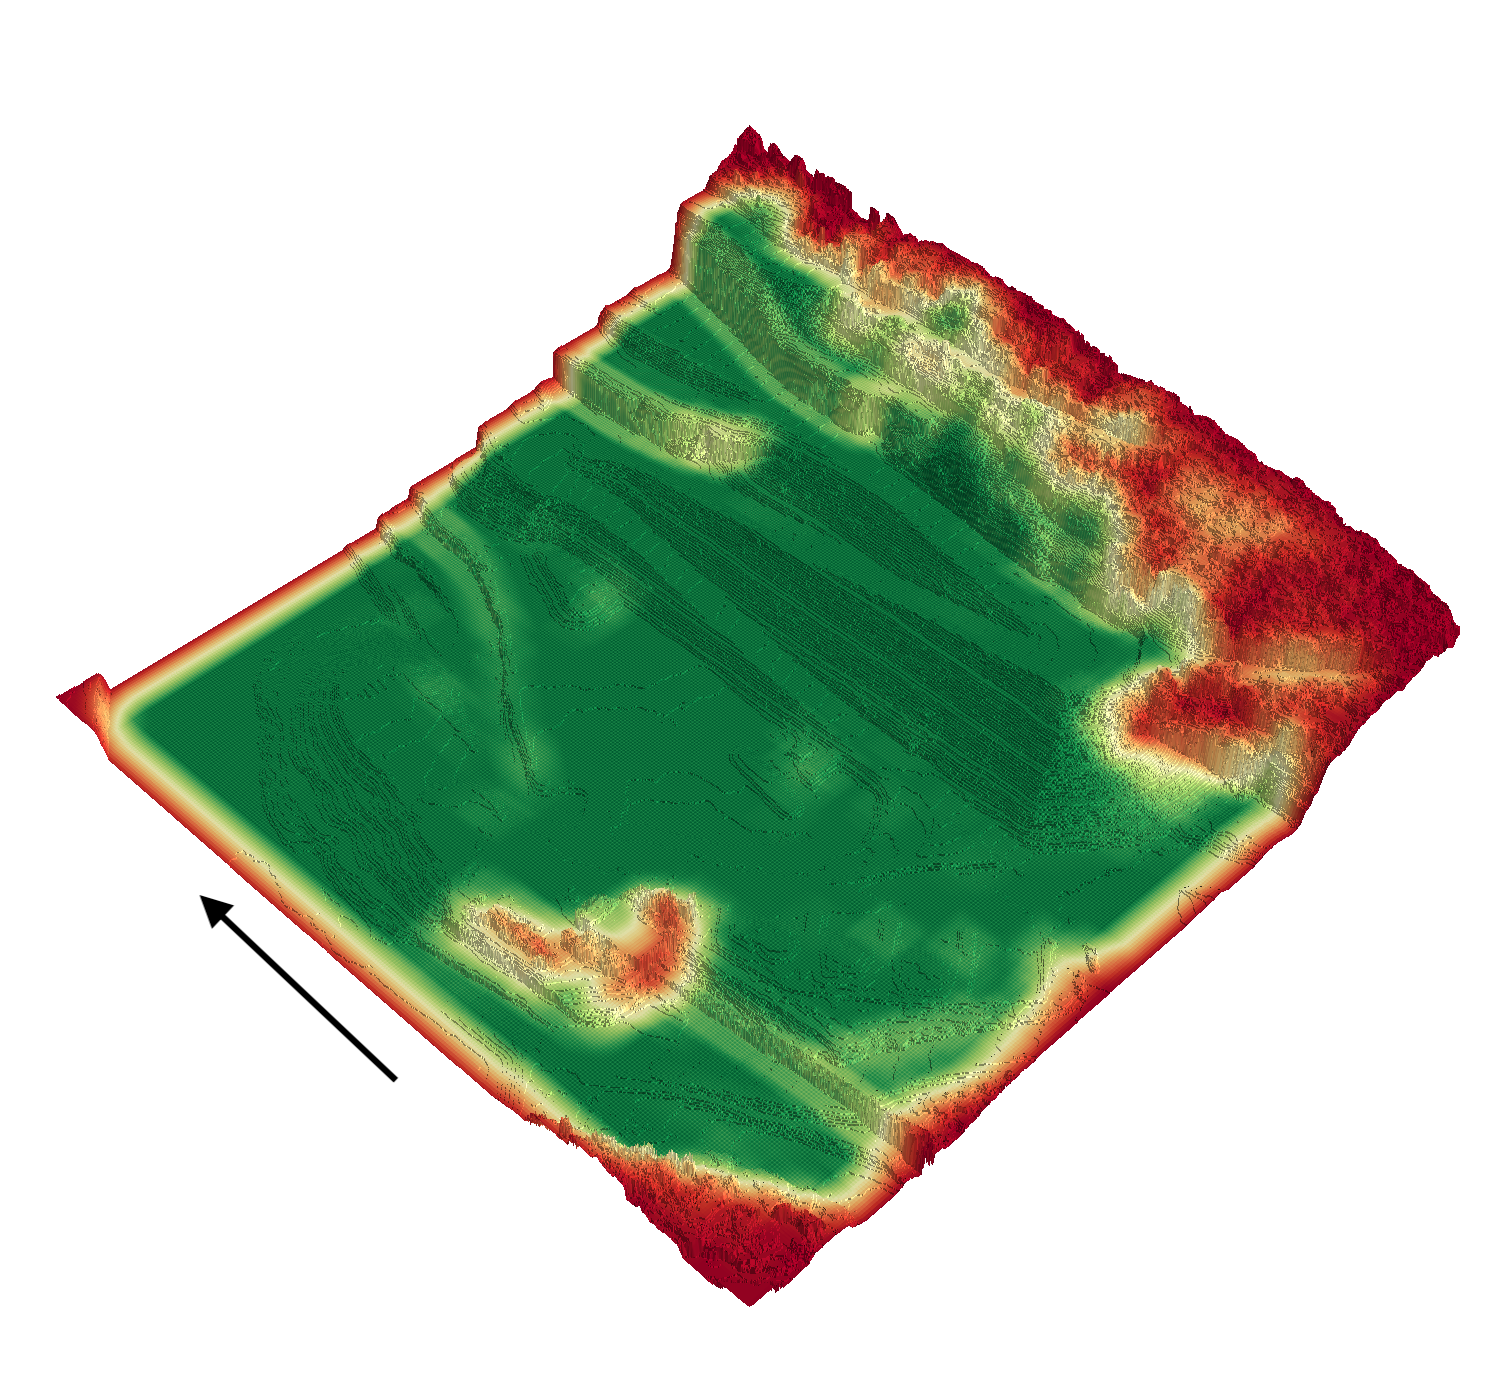
\includegraphics[width=\linewidth]{../img/4/traversability/quarry/-180.png}  
    \subcaption{Robot moving from right to left} 
    % \label{fig: quarry-r2l}
\end{subfigure}
\caption{Traversability probability on the Quarry map, $32\times 32$m, for different Krock's rotation. The values are obtained by sliding a window on the map to create the patches and then predict the traversability for each one of them.}
\end{figure}
 Correctly, the lower part of the map, composed by flat regions, was label with high confidence as traversable in all rotations. On the other hand, the traversability of the  slopes and the bumps on the top region depends on the robot orientation.
 
%  One oblious example are the slopes on then zig-zag trail. When the robot is moving up-hill, figure \ref{fig: quarry-b2t}, the propability to traverse those steep patches is low. But, if we travel down hill, figure \ref{fig: quarry-t2b}, then the slopes are traversable. This is also true, when the robot is moving from left to right and right to left, figure \ref{fig: quarry-l2r} and \ref{fig: quarry-r2l} is able to travel the slopes since the inclination is not too big to make the robot fall. 
 
\subsection{Bars}
Bars is a map composed by different heights wall, thus we expect similar probabilities with different orientation.

\begin{figure} [htbp]
  \centering
  \begin{subfigure}[b]{0.45\textwidth}
    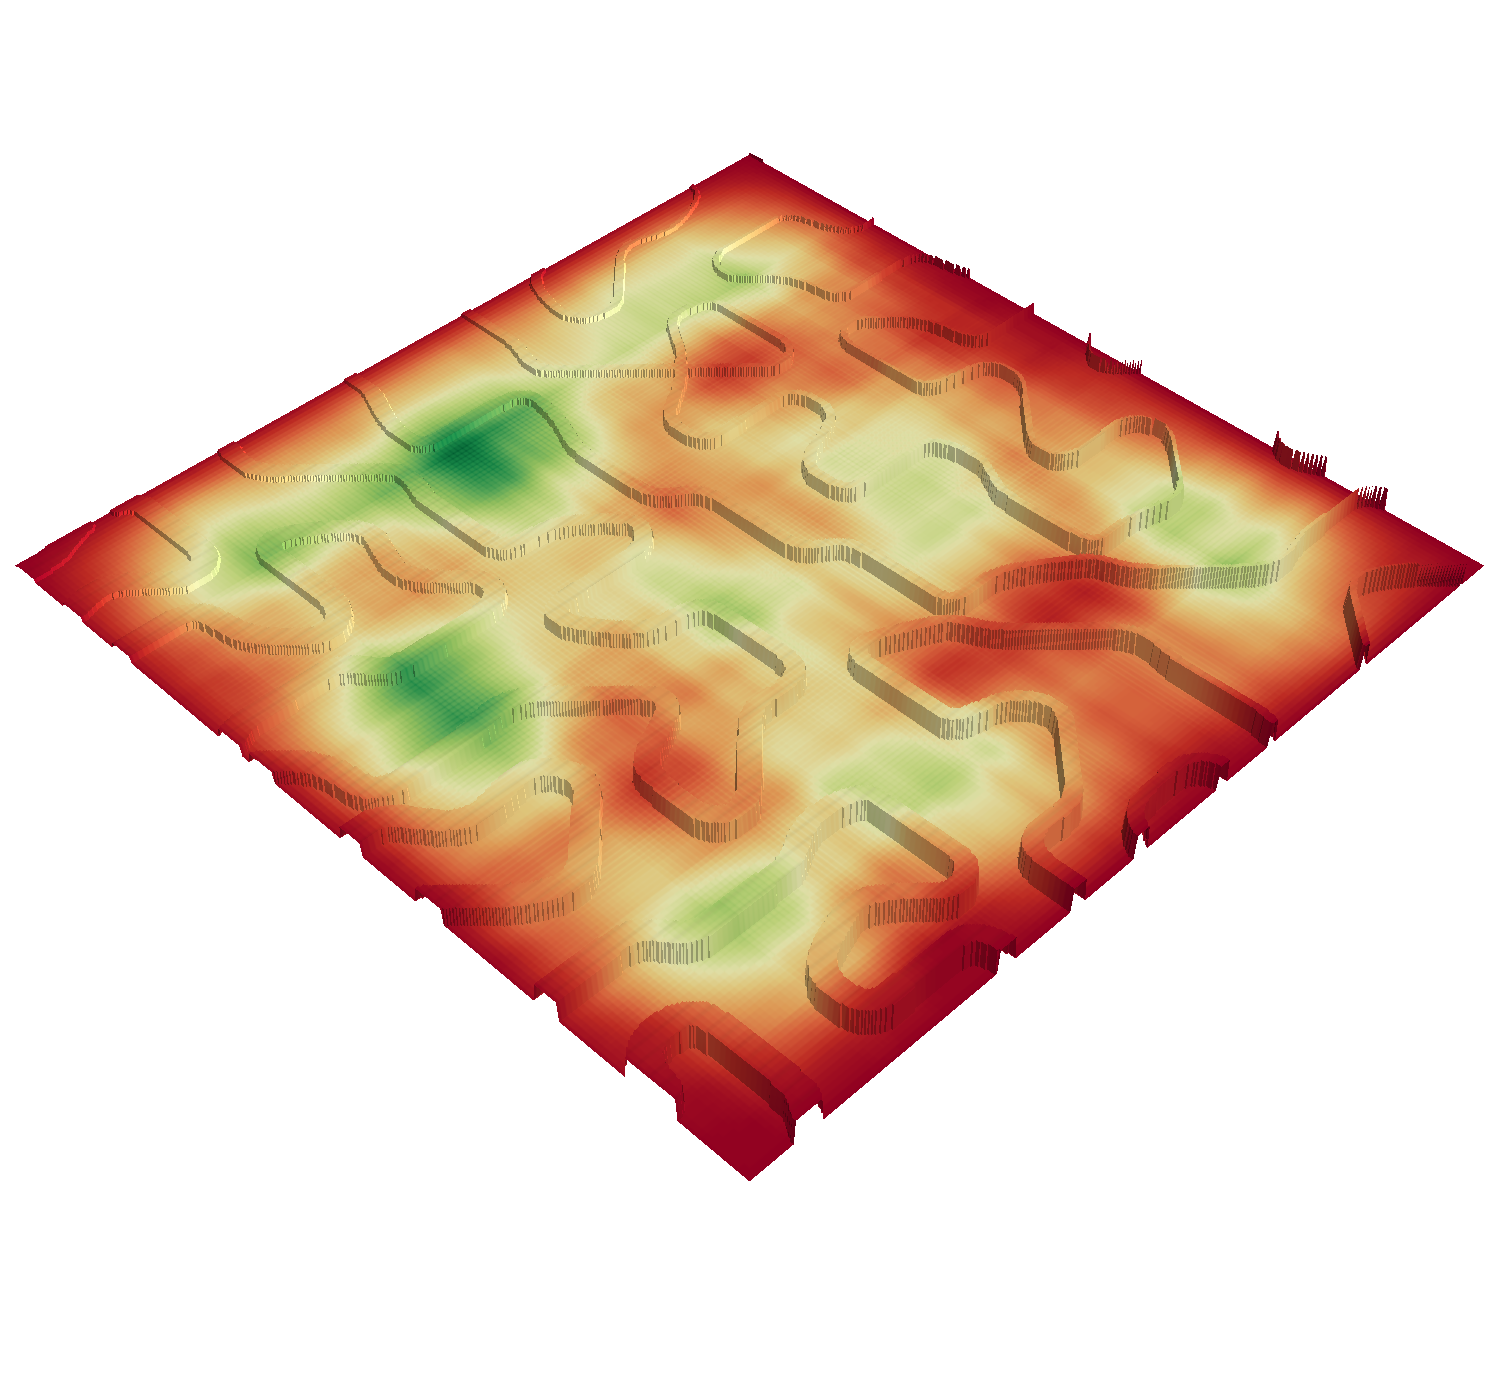
\includegraphics[width=\linewidth]{../img/4/traversability/bars/-270.png} 
    \subcaption{Robot moving from bottom to top} 
    % \label{fig: bars-b2t}
  \end{subfigure}
  \begin{subfigure}[b]{0.45\textwidth}
      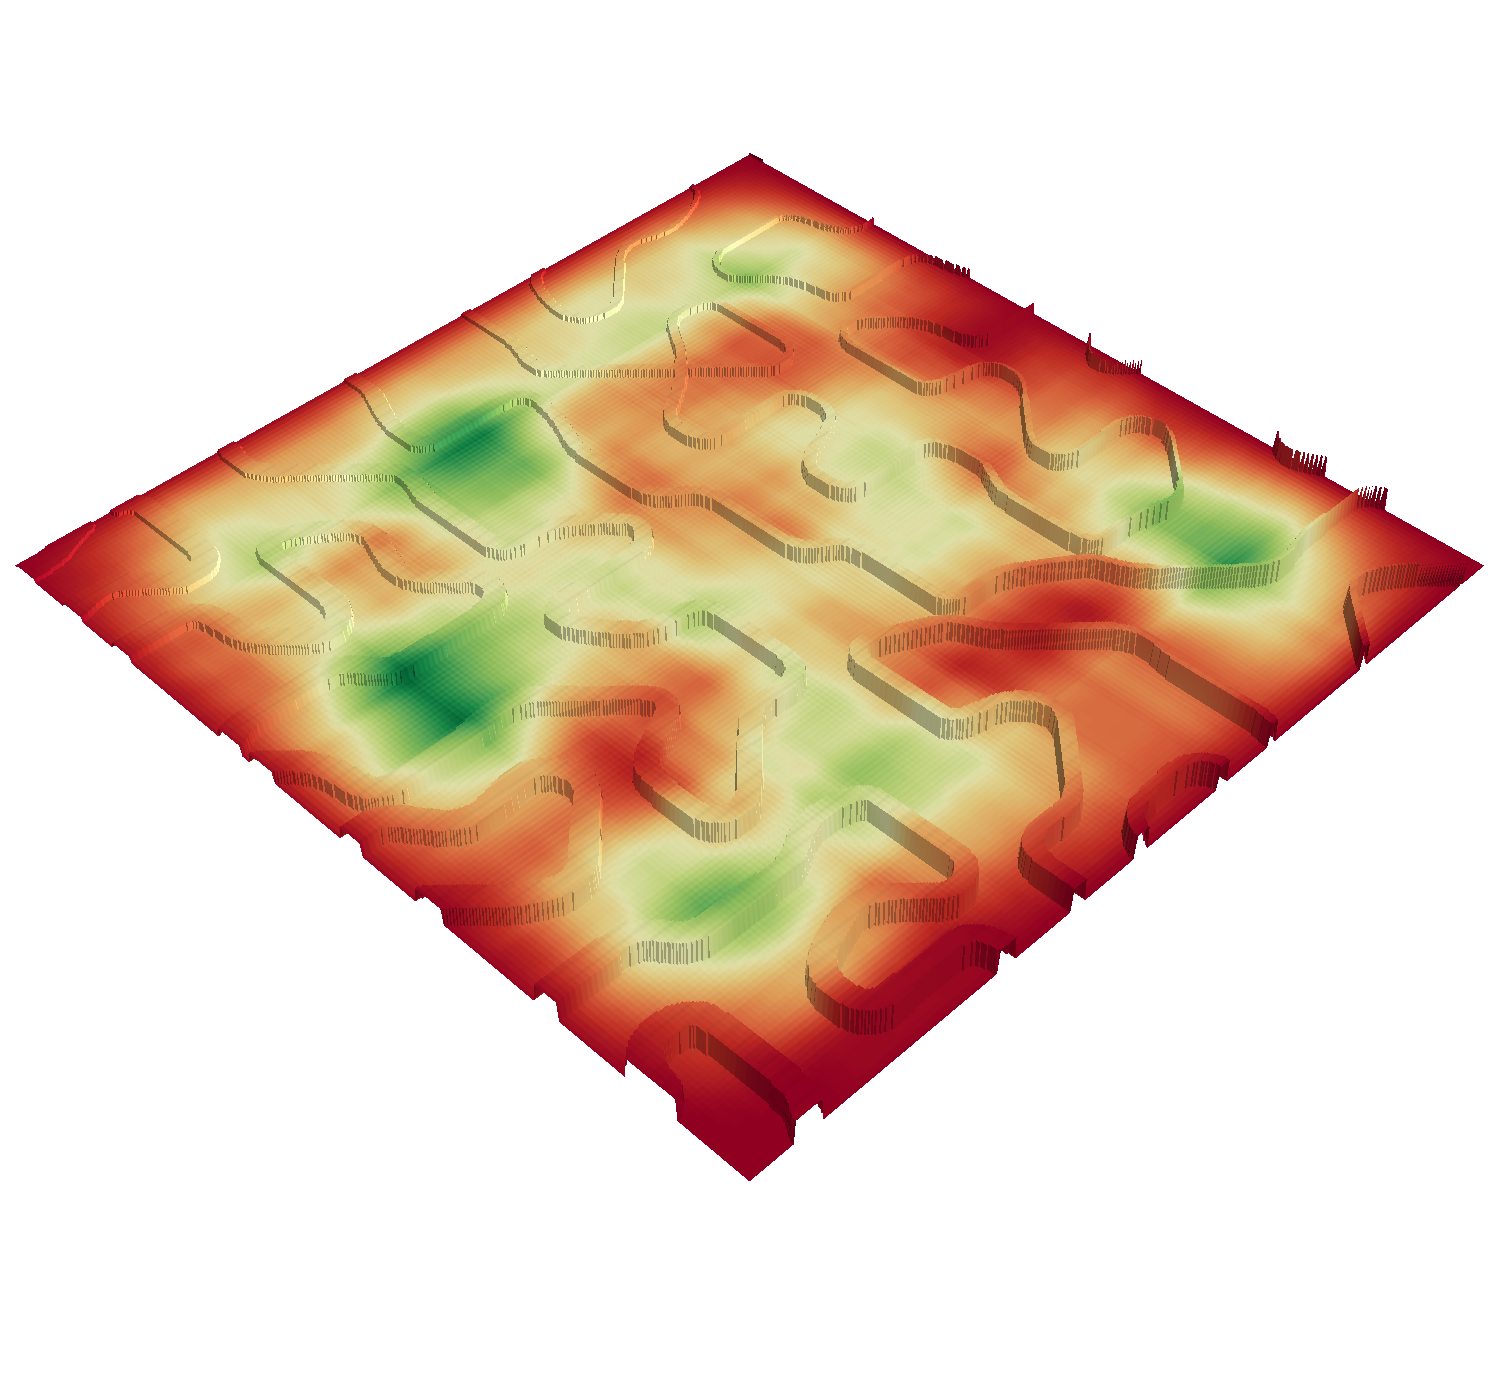
\includegraphics[width=\linewidth]{../img/4/traversability/bars/-90.png}
      \subcaption{Robot moving from top to bottom} 
      % \label{fig: bars-t2b}
  \end{subfigure}
  \begin{subfigure}[b]{0.45\textwidth}
    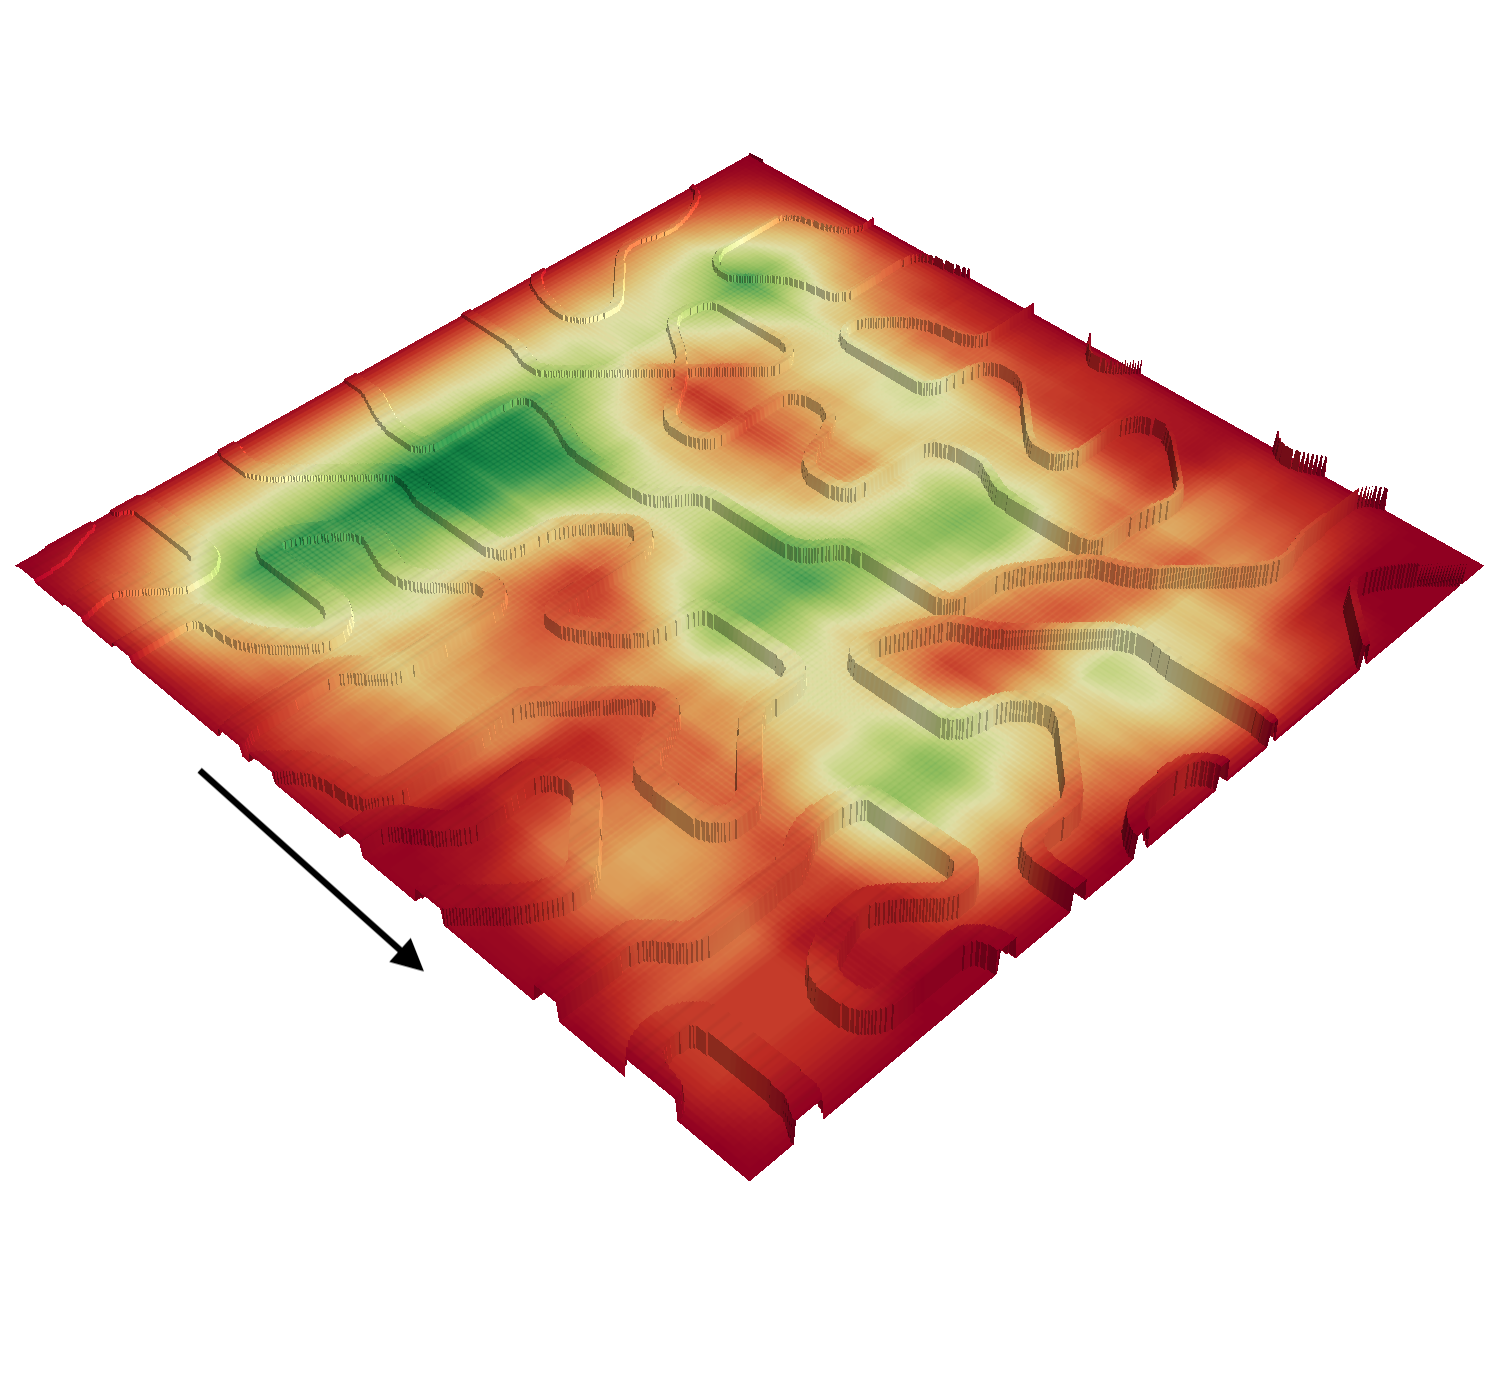
\includegraphics[width=\linewidth]{../img/4/traversability/bars/-0.png}
    \subcaption{Robot moving from left to right}   
    % \label{fig: bars-l2r}
  \end{subfigure}
  \begin{subfigure}[b]{0.45\textwidth}
      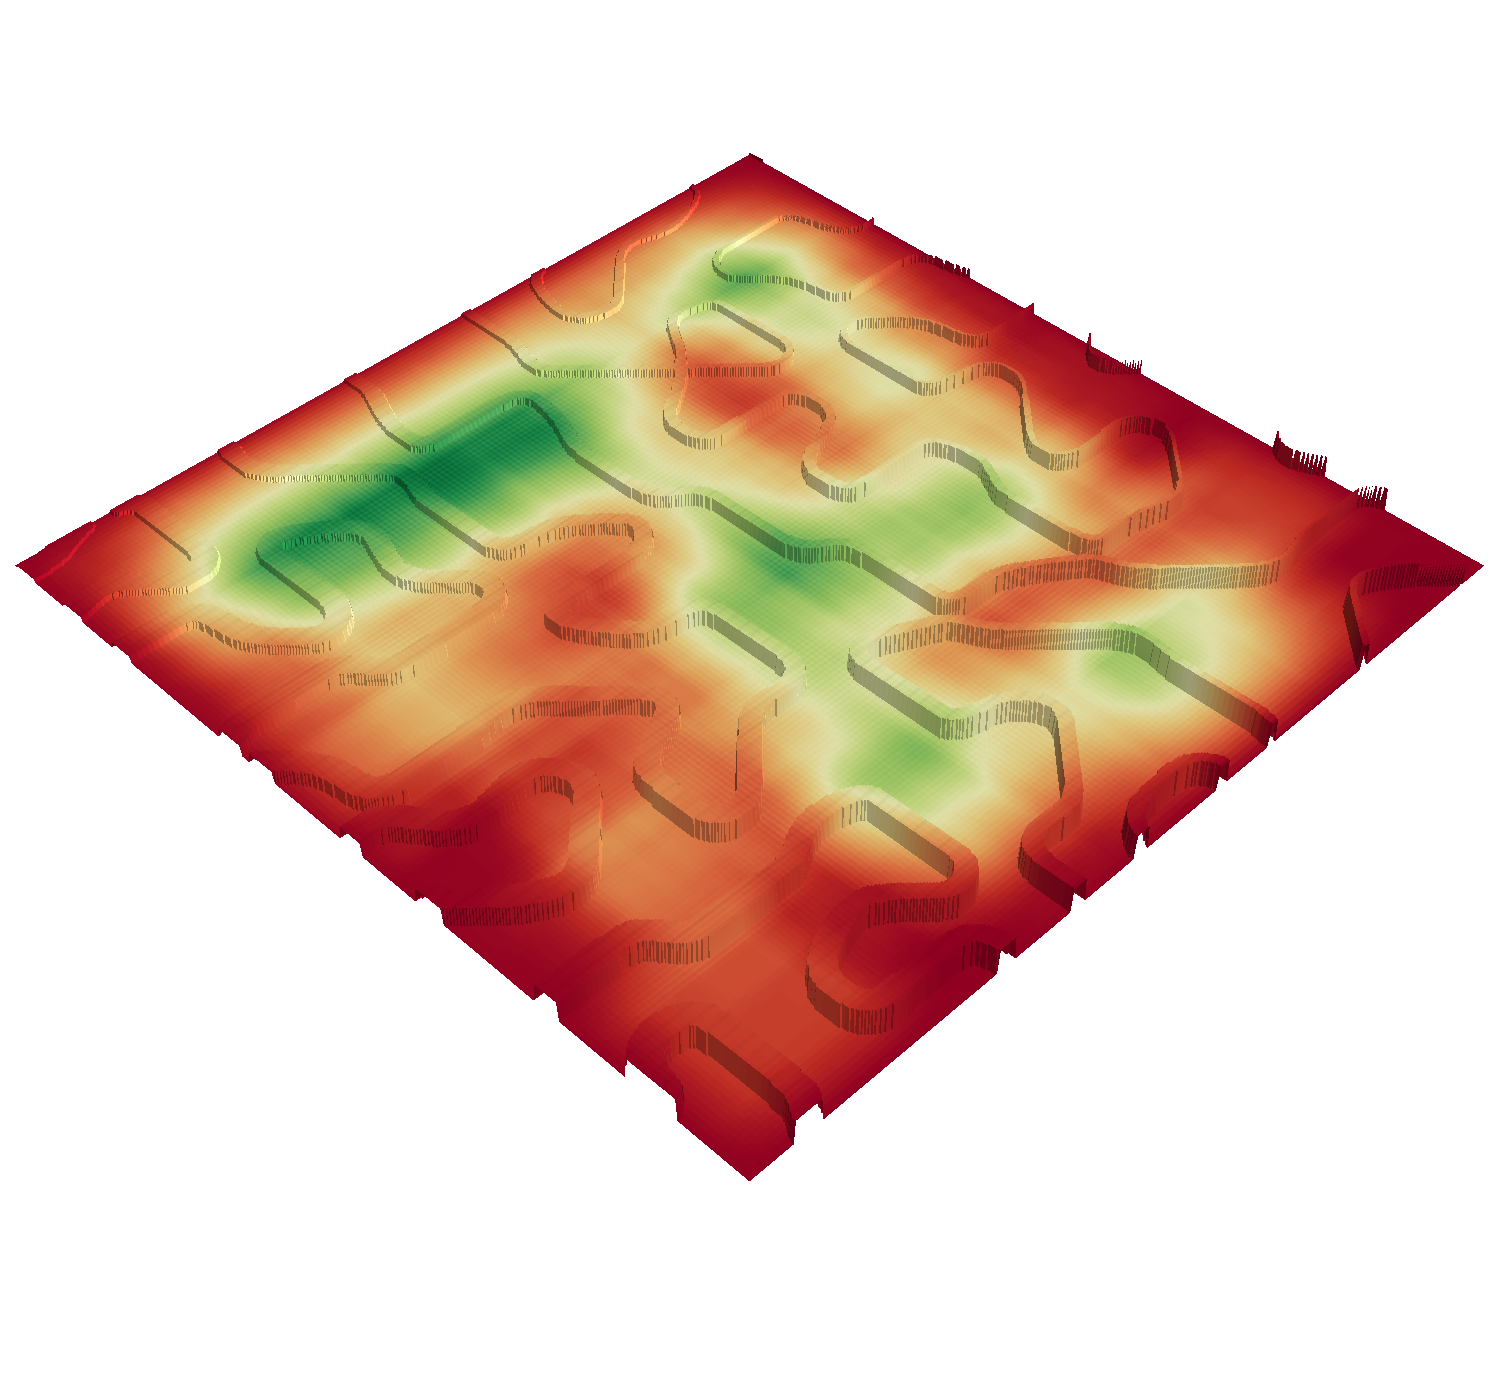
\includegraphics[width=\linewidth]{../img/4/traversability/bars/-180.png}  
      \subcaption{Robot moving from right to left} 
      % \label{fig: bars-r2l}
  \end{subfigure}
  \caption{Traversability probability on the bars map, $10\times 10$m, for different Krock's rotation. The values are obtained by sliding a window on the map to create the patches and then predict the traversability for each one of them.}
  \end{figure}

This is a hard map for the robot due to the high number of not traversable walls. Interesting, we can identify a tunnel near the bottom center of the maps that shows how the model correctly label those patches depending on the orientation. The following figure highlight this detail.

\begin{figure} [htbp]
  \centering
  \begin{subfigure}[b]{0.23\textwidth}
    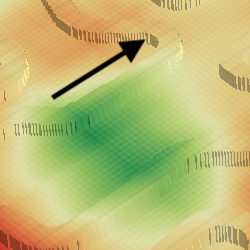
\includegraphics[width=\linewidth]{../img/4/traversability/bars/tunnel/-270-crop.png} 
    % \subcaption{Robot moving from bottom to top} 
    % \label{fig: bars-b2t}
  \end{subfigure}
  \begin{subfigure}[b]{0.23\textwidth}
      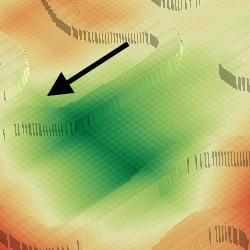
\includegraphics[width=\linewidth]{../img/4/traversability/bars/tunnel/-90-crop.png}
      % \subcaption{Robot moving from top to bottom} 
      % \label{fig: bars-t2b}
  \end{subfigure}
  \begin{subfigure}[b]{0.23\textwidth}
    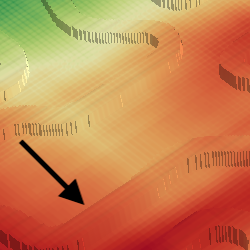
\includegraphics[width=\linewidth]{../img/4/traversability/bars/tunnel/-0-crop.png}
    % \subcaption{Robot moving from left to right}   
    % \label{fig: bars-l2r}
  \end{subfigure}
  \begin{subfigure}[b]{0.23\textwidth}
      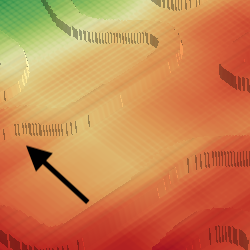
\includegraphics[width=\linewidth]{../img/4/traversability/bars/tunnel/-180-crop.png}  
      % \subcaption{Robot moving from right to left} 
      % \label{fig: bars-r2l}
  \end{subfigure}
  \caption{Detail of a region in the bars map where there are two walls forming a tunnel. Correctly, when the robot is travel following the trail the region is label as traversable.}
  \end{figure}

\subsection{Small village}
The following image shows the traversability probability on the small image map.

\begin{figure} [htbp]
  \centering
  \begin{subfigure}[b]{0.45\textwidth}
    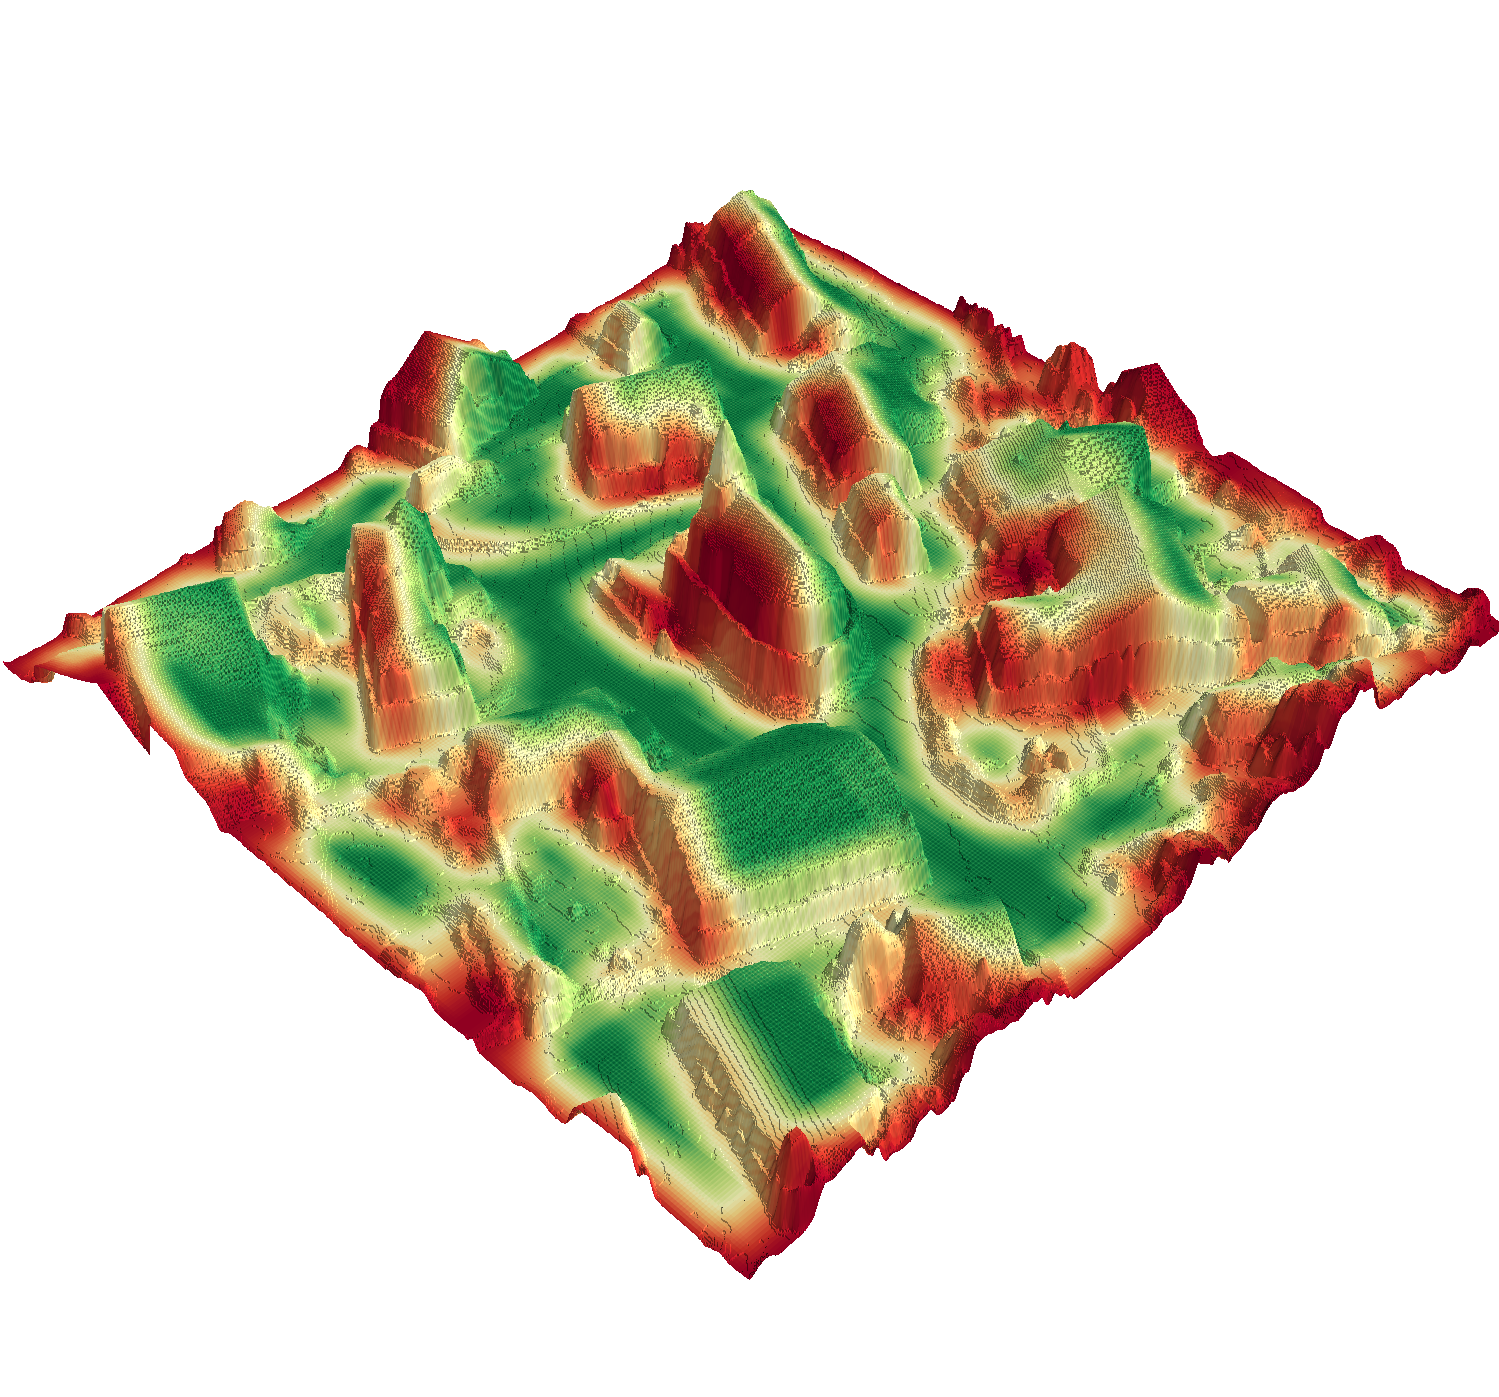
\includegraphics[width=\linewidth]{../img/4/traversability/sullens/-270.png} 
    \subcaption{Robot moving from bottom to top} 
    % \label{fig: sullens-b2t}
  \end{subfigure}
  \begin{subfigure}[b]{0.45\textwidth}
      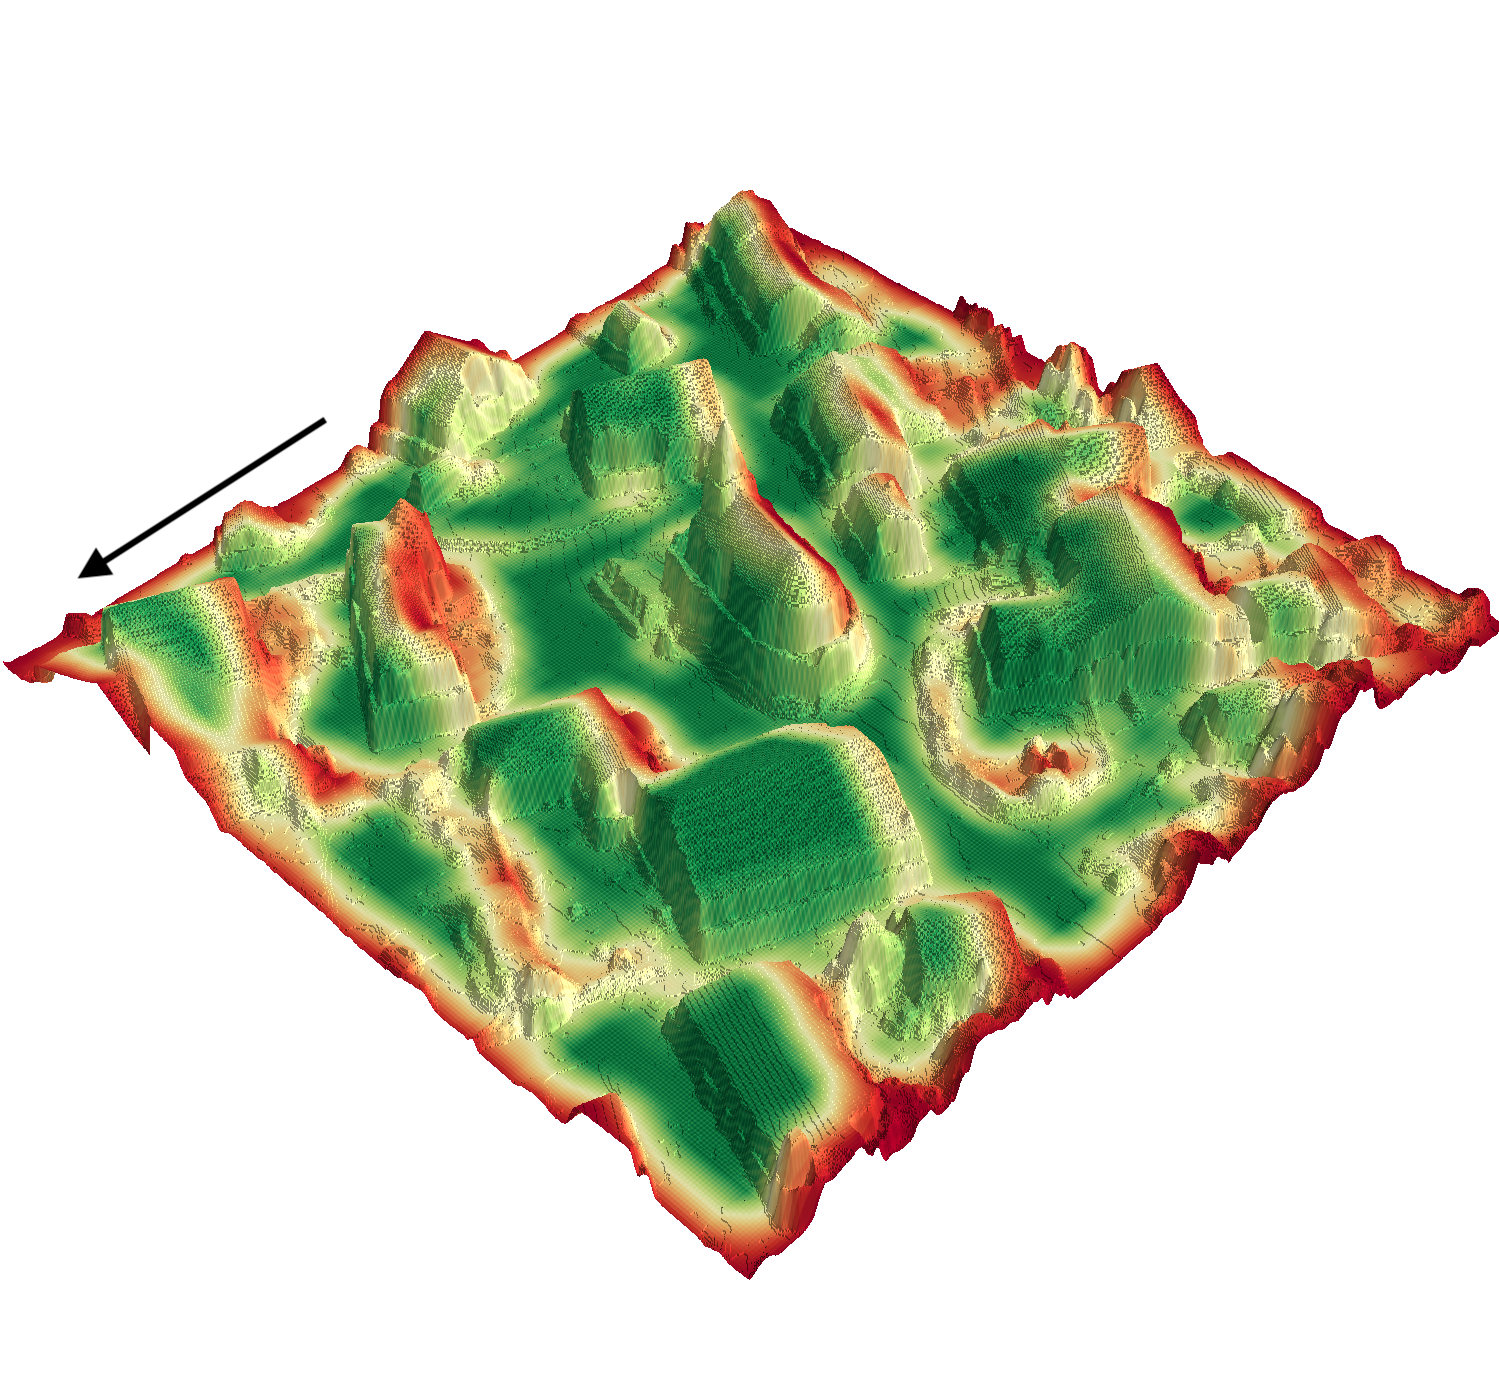
\includegraphics[width=\linewidth]{../img/4/traversability/sullens/-90.png}
      \subcaption{Robot moving from top to bottom} 
      % \label{fig: sullens-t2b}
  \end{subfigure}
  \begin{subfigure}[b]{0.45\textwidth}
    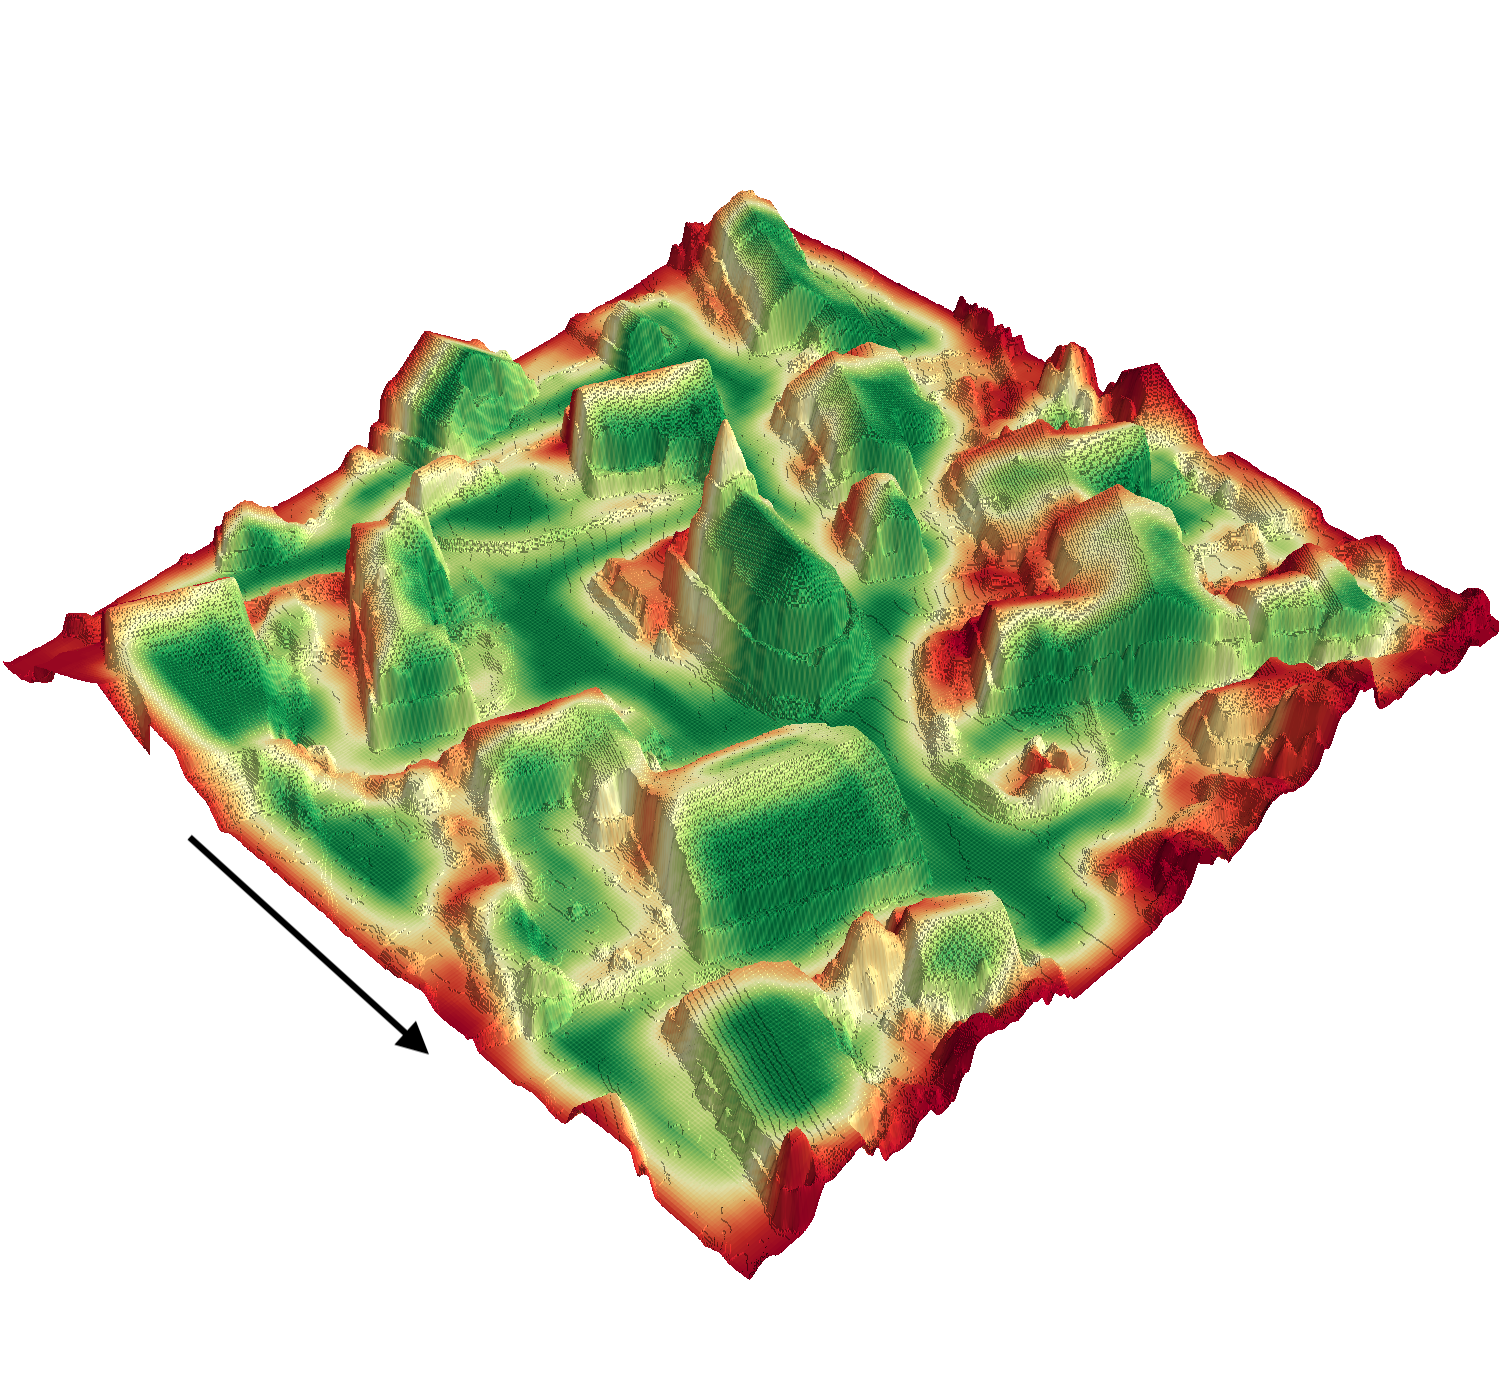
\includegraphics[width=\linewidth]{../img/4/traversability/sullens/-0.png}
    \subcaption{Robot moving from left to right}   
    % \label{fig: sullens-l2r}
  \end{subfigure}
  \begin{subfigure}[b]{0.45\textwidth}
      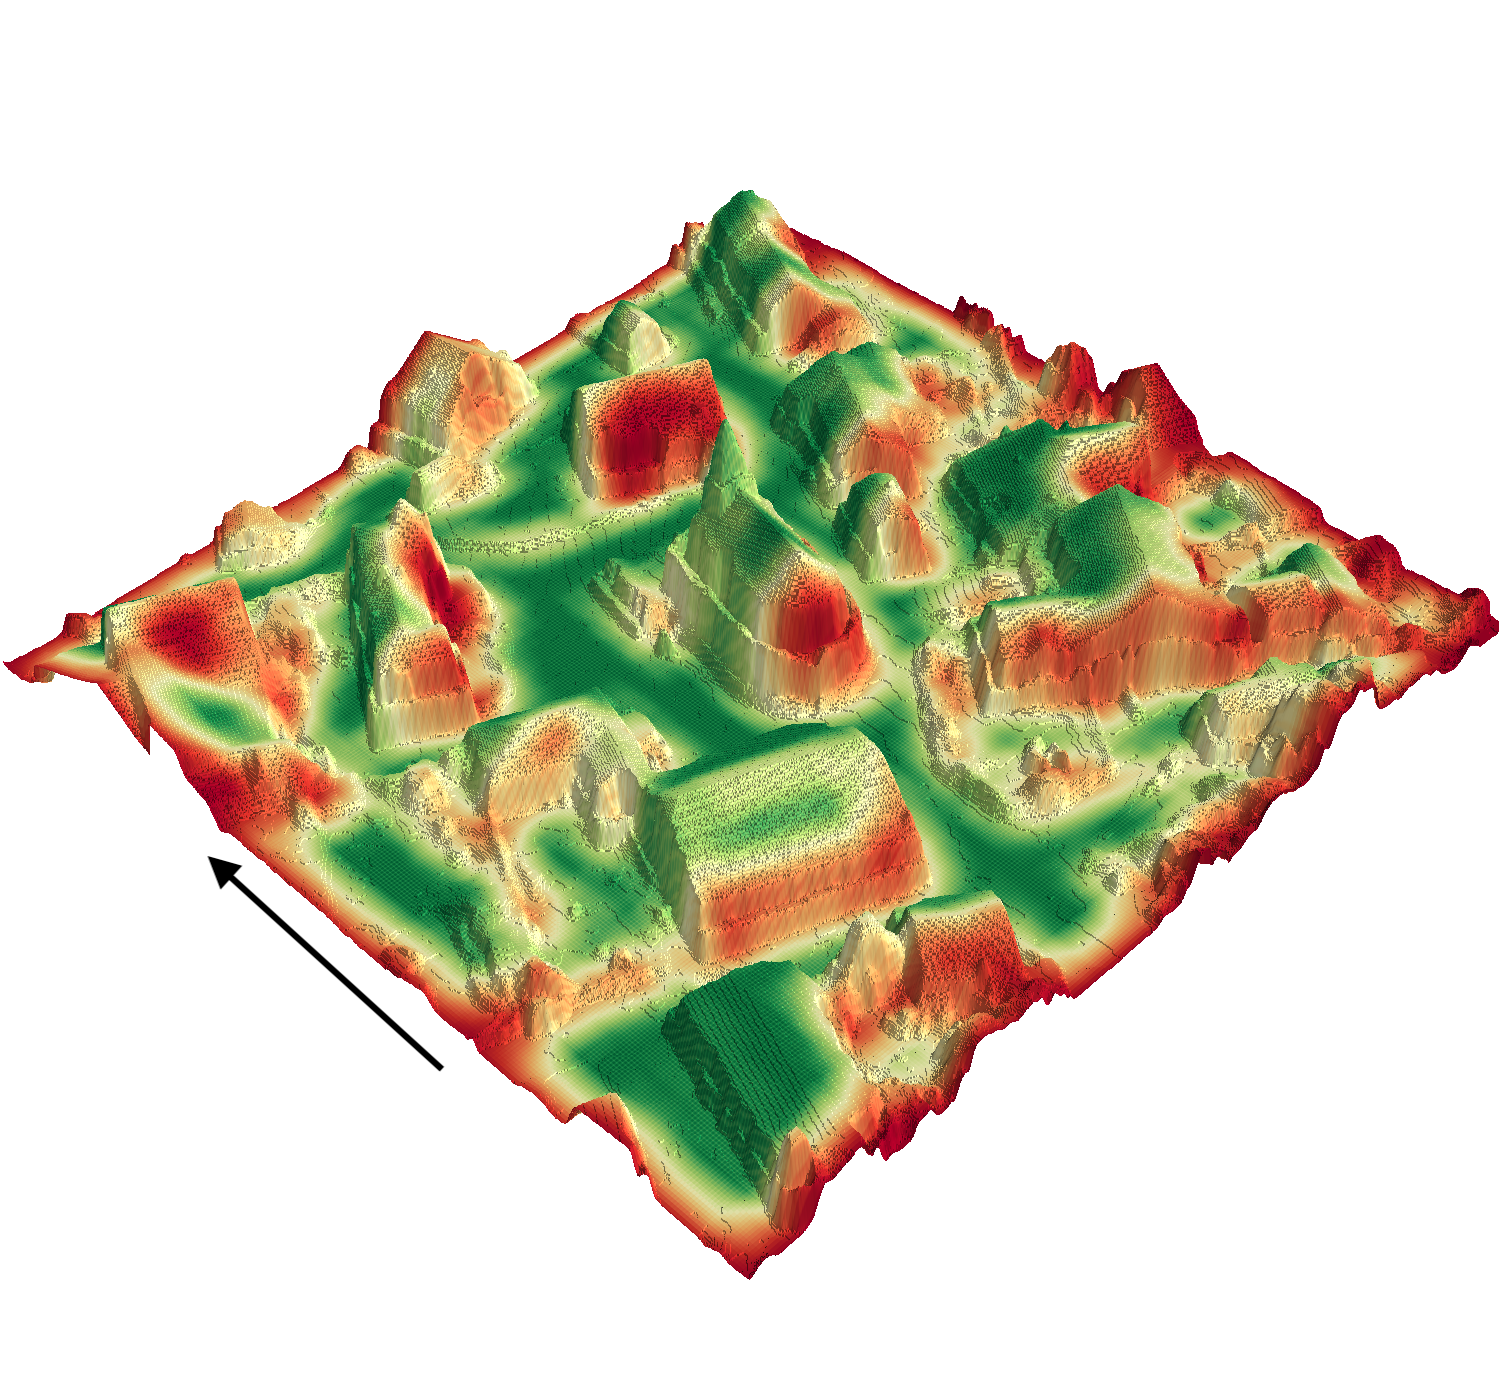
\includegraphics[width=\linewidth]{../img/4/traversability/sullens/-180.png}  
      \subcaption{Robot moving from right to left} 
      % \label{fig: bars-r2l}
  \end{subfigure}
  \caption{Traversability probability on the map of a small village for different Krock's rotation. The surface cover $30\times 30$m and has a maximum height of $10$m. The values are obtained by sliding a window on the map to create the patches and then predict the traversability for each one of them.}
  \end{figure}
  All the streest were label as traversble, while the roofs' traversability depend on the orientation. For example, most steep roofs are not traversble when walking up hill. On the other hand, if krock walk side by side they can be traverse. The following figure shows this behaviour on the church's roof.
  \begin{figure} [htbp]
    \centering
    \begin{subfigure}[b]{0.45\textwidth}
      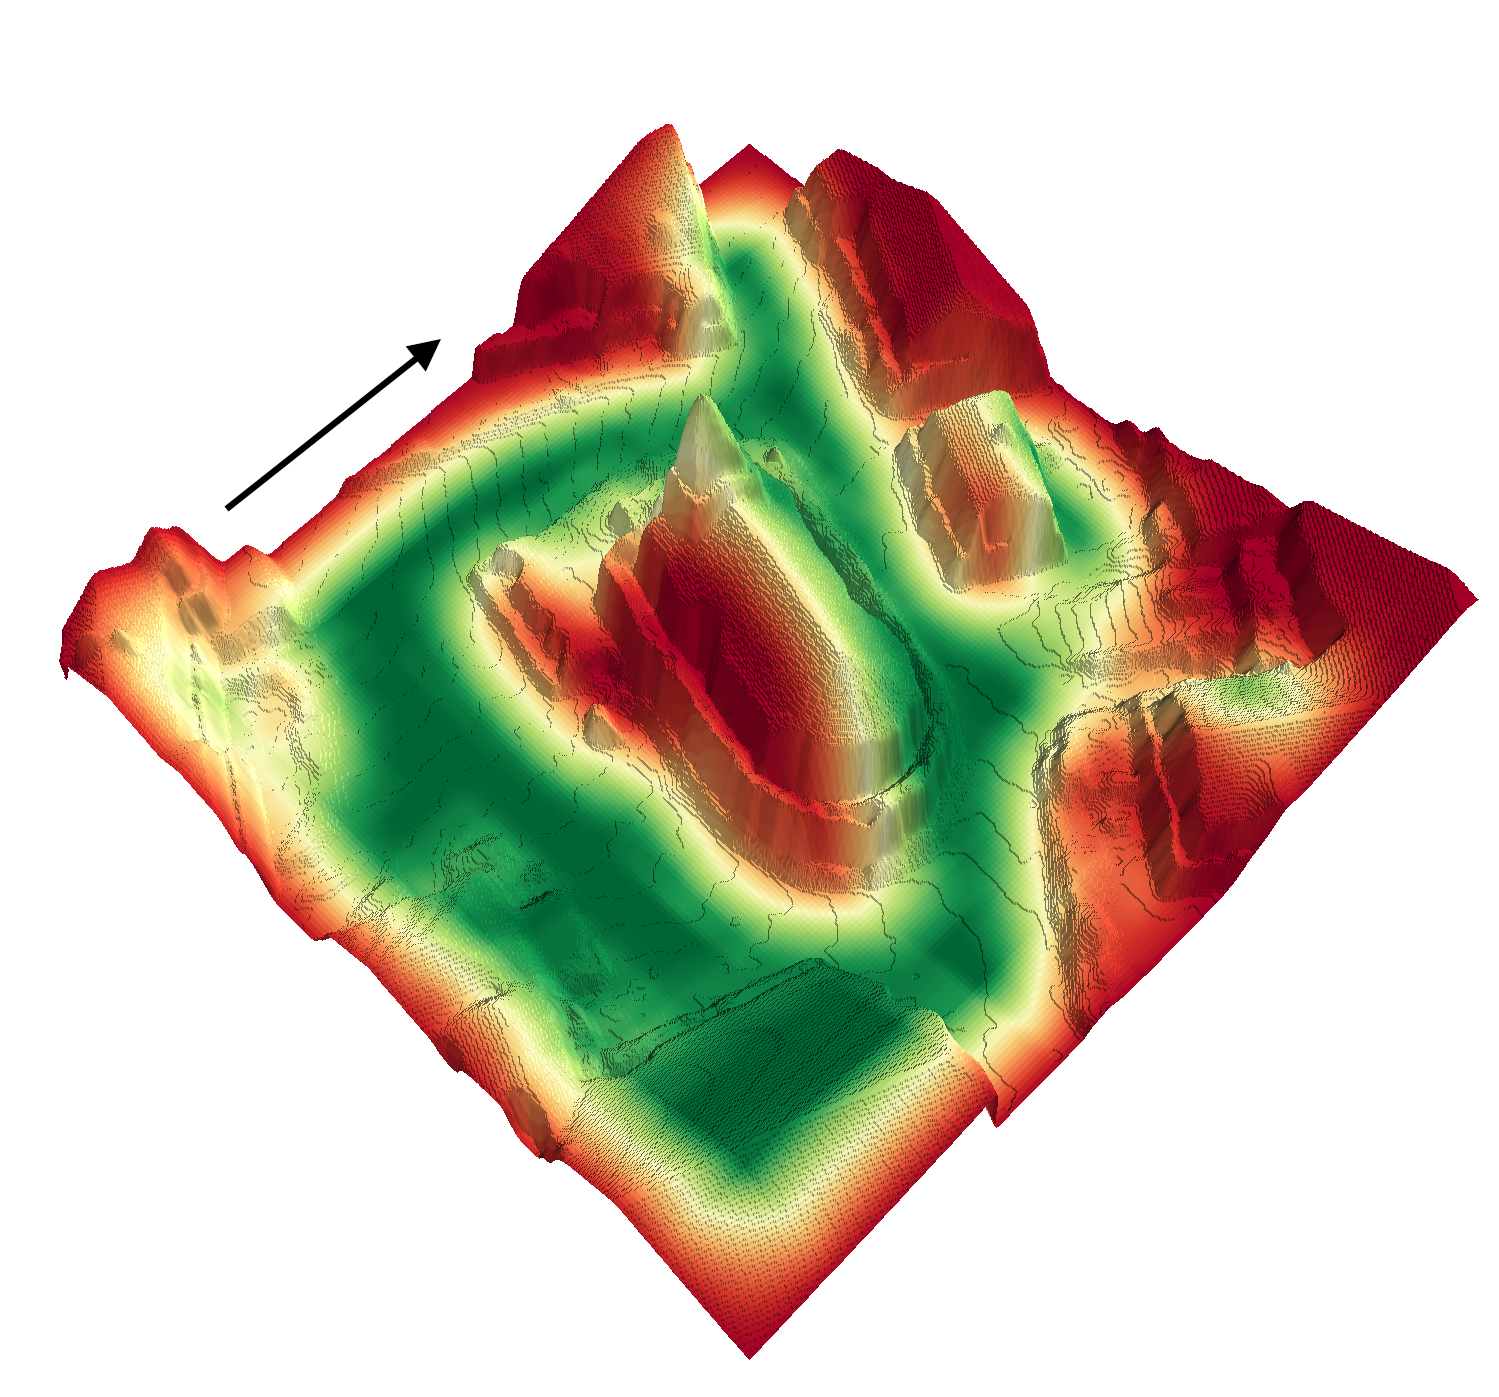
\includegraphics[width=\linewidth]{../img/4/traversability/sullens-church/-270.png} 
      \subcaption{Robot moving from bottom to top} 
      % \label{fig: sullens-b2t}
    \end{subfigure}
    \begin{subfigure}[b]{0.45\textwidth}
        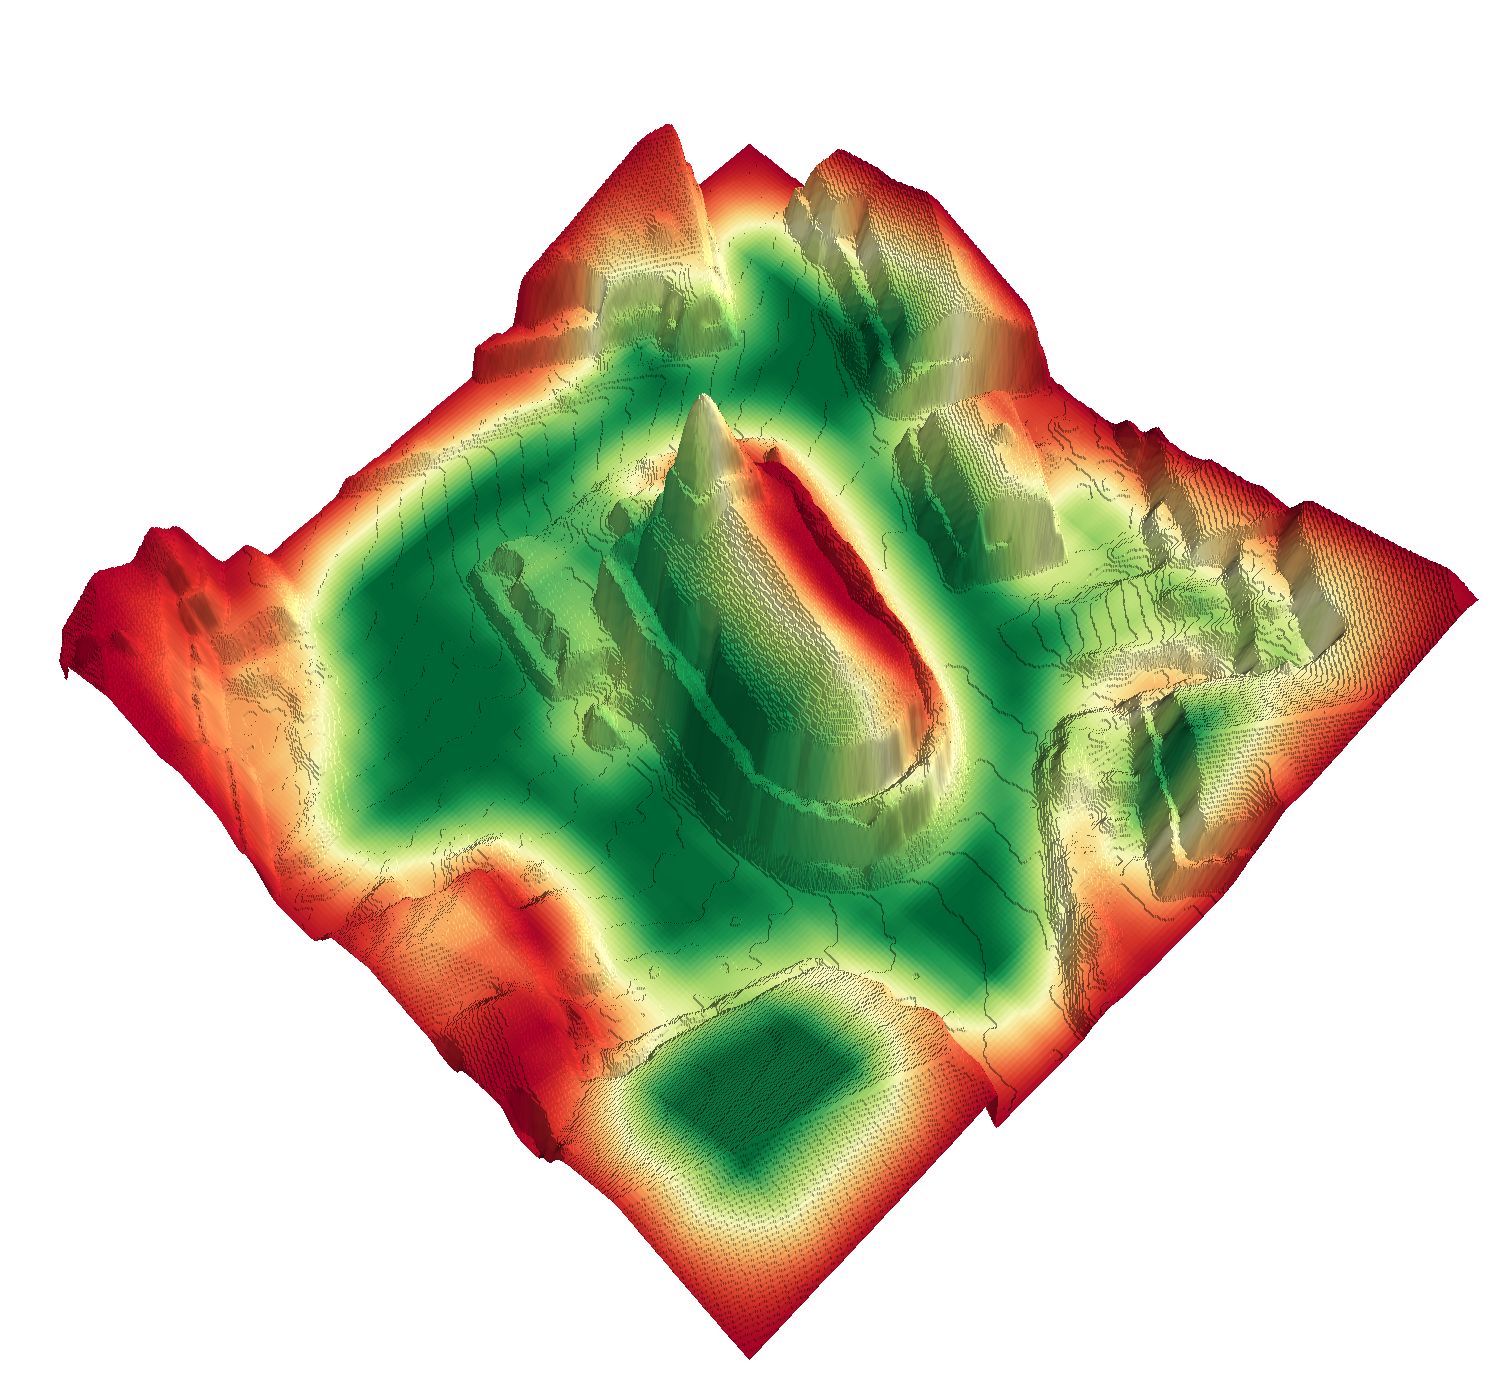
\includegraphics[width=\linewidth]{../img/4/traversability/sullens-church/-90.png}
        \subcaption{Robot moving from top to bottom} 
        % \label{fig: sullens-church-t2b}
    \end{subfigure}
    \begin{subfigure}[b]{0.45\textwidth}
      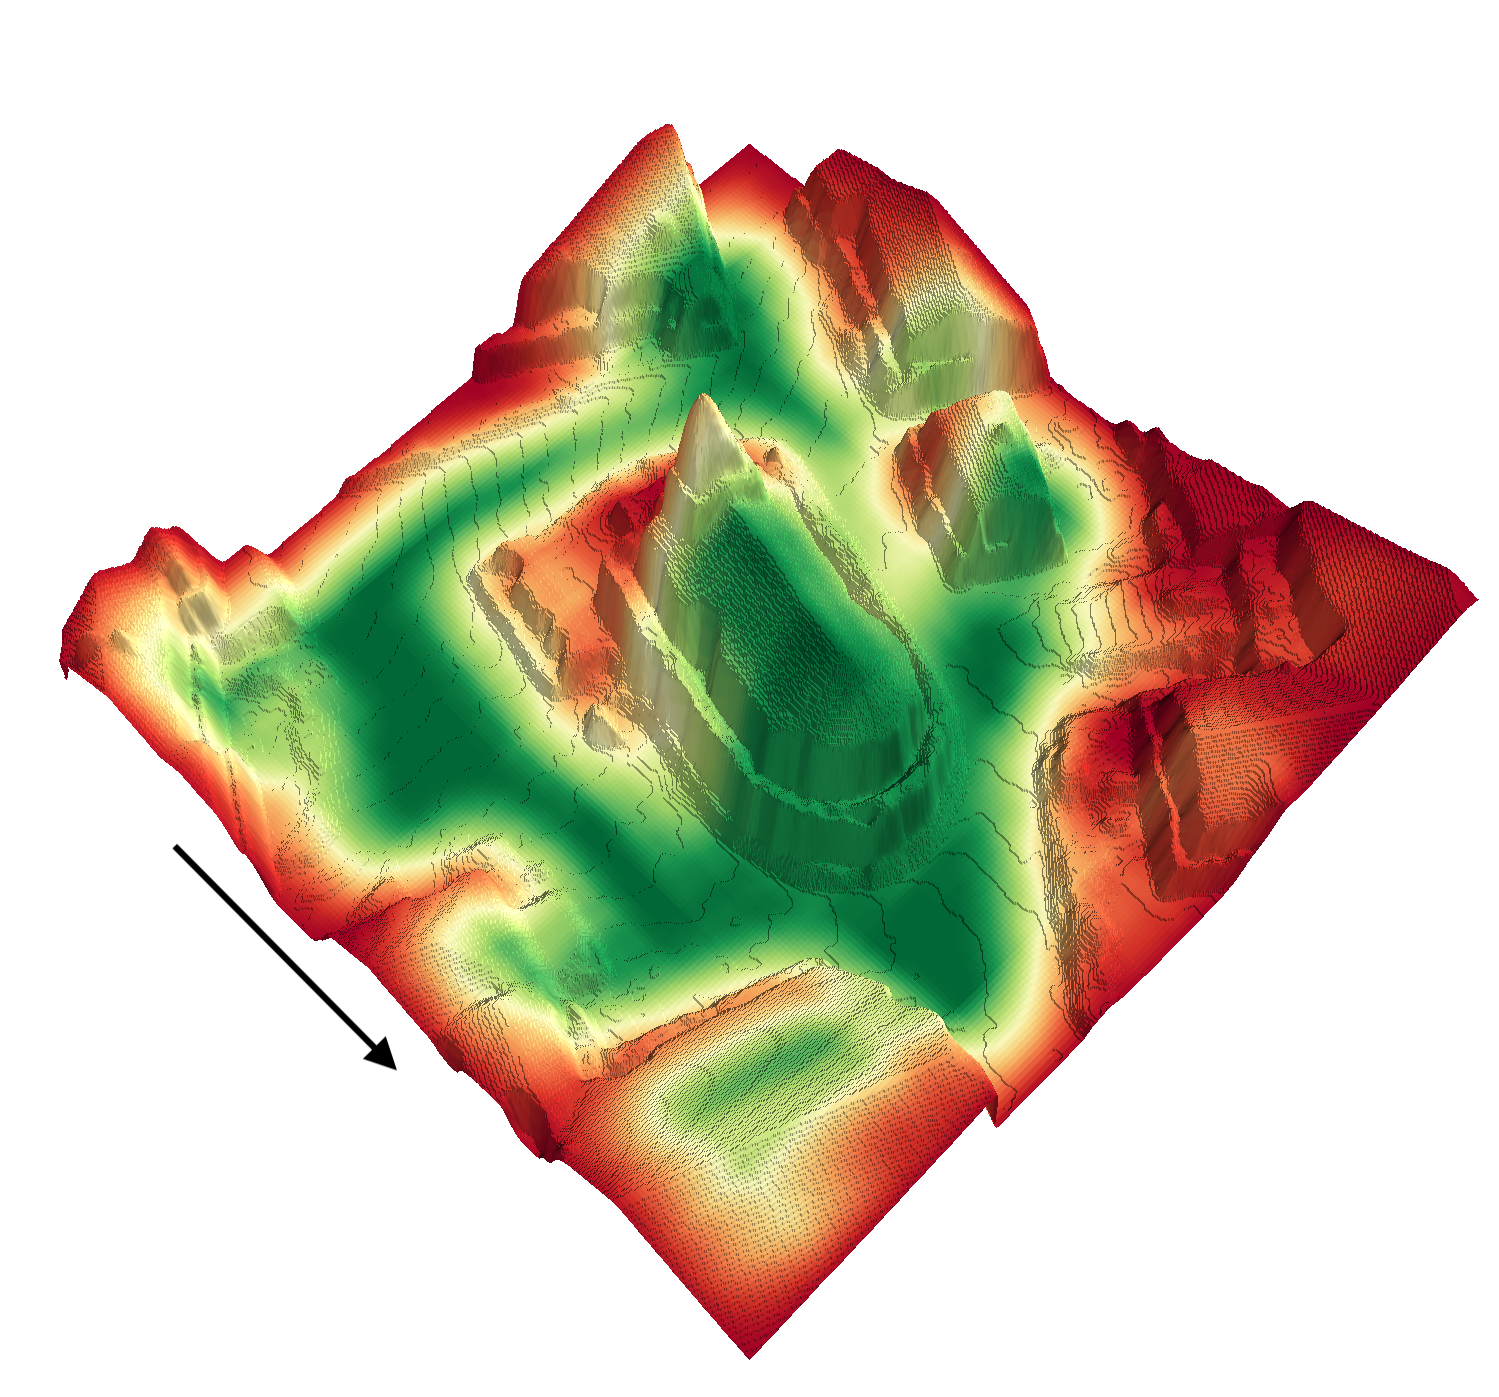
\includegraphics[width=\linewidth]{../img/4/traversability/sullens-church/-0.png}
      \subcaption{Robot moving from left to right}   
      % \label{fig: sullens-church-l2r}
    \end{subfigure}
    \begin{subfigure}[b]{0.45\textwidth}
        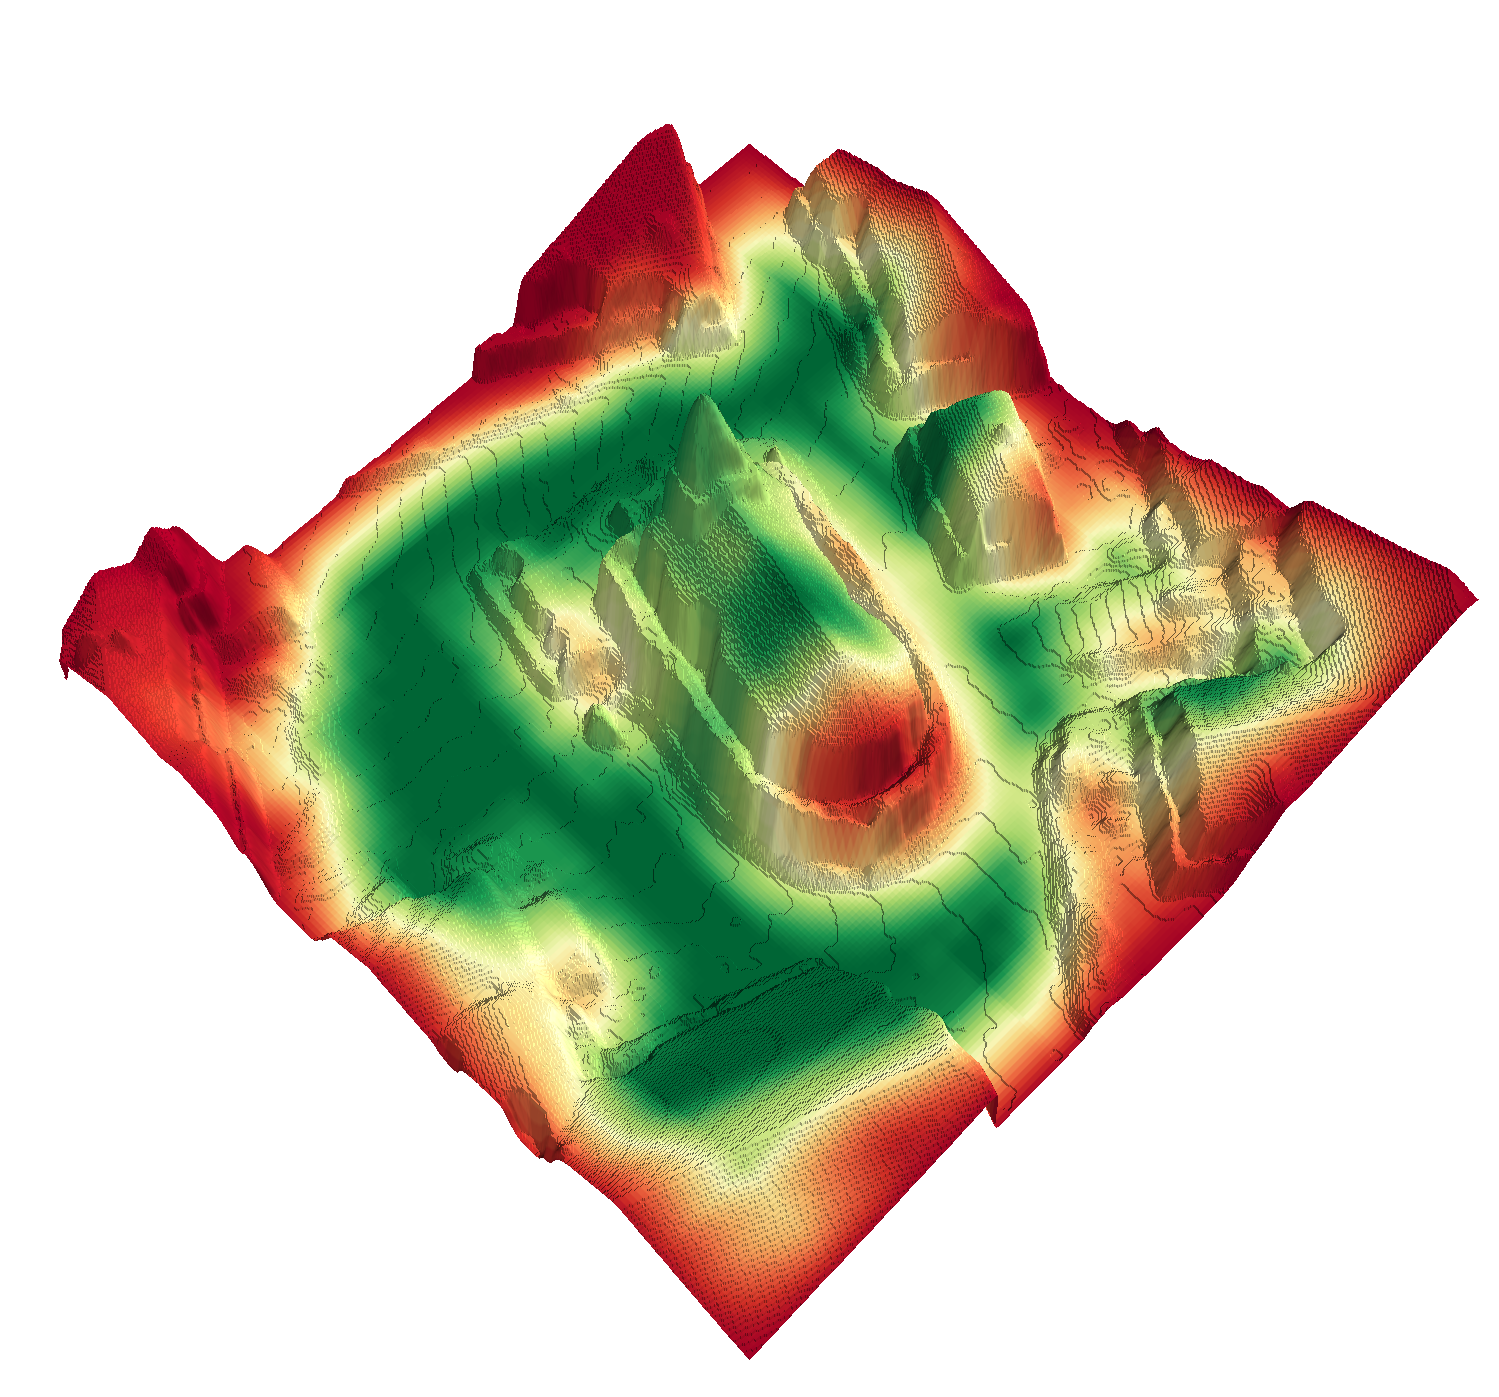
\includegraphics[width=\linewidth]{../img/4/traversability/sullens-church/-180.png}  
        \subcaption{Robot moving from right to left} 
        % \label{fig: bars-r2l}
    \end{subfigure}
    \caption{Detail of the church in the small village map for different Krock's rotation. We can notice for the first two image one part of the roof is traversable and vicevera. While for the last two the robot can correctly travel til the end.}
    \end{figure}
\end{document}